\documentclass[11pt]{article}

\usepackage[letterpaper,margin=1in]{geometry}
\usepackage{amsmath}
\usepackage{array}
\usepackage{booktabs}
\usepackage{caption}
\usepackage{enumitem}
\usepackage{float}
\usepackage{graphicx}
\usepackage{hyperref}
\usepackage{lineno}
\usepackage{listings}
\usepackage{longtable}
\usepackage{xcolor}

\graphicspath{{figures/}}
\hypersetup{
  colorlinks=true,
  linkcolor=black,
  citecolor=black,
  urlcolor=blue
}
\setlength{\parindent}{1.2em}
\setlength{\parskip}{0pt}
\setlist[enumerate]{leftmargin=*, itemsep=0.25em}
\newcolumntype{L}[1]{>{\raggedright\arraybackslash}p{#1}}
\captionsetup{font=small, labelfont=bf}
\lstset{
  basicstyle=\ttfamily\footnotesize,
  breaklines=true,
  frame=single,
  columns=fullflexible,
  keepspaces=true,
  backgroundcolor=\color[HTML]{F7F5EF}
}
\sloppy

\title{Is more thinking always better? Think again:\\
Model-cognition fit in AI-supported sensory analysis}
\author{
John M. Ennis\thanks{Corresponding author: john.m.ennis@aigora.com}\\
Aigora, Richmond, Virginia, USA
\and
Thierry Worch\\
FrieslandCampina, Wageningen, The Netherlands
\and
Benjamin Mahieu\\
Oniris, Nantes, France
}
\date{August 2026}

\begin{document}
\linenumbers
\maketitle

\begin{abstract}
Large language models (LLMs) can score open-ended consumer text, and many
current systems expose a configurable \emph{thinking} setting: an inference
option that spends extra compute on intermediate reasoning before the model
returns a final answer. More deliberative settings are often assumed to score
better. We tested that assumption on the published Ideal-Free-Comment study in
which 483 French consumers evaluated 30 commercial cooked hams at home (2,758
evaluations), describing each product and their ideal ham in their own words
while also rating liking. Using typical fast commercial models from one family
available at the time of the experiment,
we compared each consumer's actual and ideal Free-Comment descriptions and
returned structured alignment scores for visual appearance, texture, and
flavor, which were then used to predict liking under consumer-group holdout.
Across 27 configurations that varied direct-response versus thinking level,
response scale size, and temperature, a direct-response setup predicted liking
best ($R^2 = 0.573$), clearly above a generic embedding-similarity baseline.
Setups with thinking turned on, from a related generation in the same family,
were slower and did not close that gap. In a controlled comparison at six scale
points and temperature 0.7, they were also less reliable at returning parseable
structured output. Within that thinking-capable generation, low thinking
improved prediction and structured-output reliability over minimal thinking
but substantially increased runtime. The alignment scores recovered the
published sensory modality hierarchy and, in a held-out construct check,
recovered Just-About-Right ratings the model never saw, attribute by
attribute; thinking settings did not improve that recovery. These results
come from one model family (Gemini fast commercial models available when we
ran the experiment). They are not general laws about all LLMs. The point of
the paper is that thinking level matters for sensory text scoring, and that it
can matter in a surprising way: more deliberation was not automatically
better. A careful analogy to ideas about fast versus more deliberate human
judgment offers one way to think about why that pattern might arise. The
human brain is far more complex than any current LLM, but the parallel may
help frame new work in sensometrics. Readers should treat our findings as a
prompt to try thinking settings on their own tasks, whether they use closed
or open models.
\end{abstract}

\noindent\textbf{Keywords:} Free-Comment; Ideal-Free-Comment; sensory analysis;
consumer liking; large language models; model-cognition fit.

\section{Introduction}
\label{sec:intro}

Consumer sensory research needs to measure how products compare with what
consumers actually want, and it needs to do so at scale. Structured elicitation
methods such as Check-All-That-Apply (CATA), Just-About-Right (JAR) scales, and
the Ideal Profile Method (IPM) give analysts clean tables, but they impose a
vocabulary in advance [Worch et al., 2013]. Free-Comment methods do the
opposite. They let consumers use their own words, which brings the data closer
to the consumer's own experience while avoiding vocabulary restriction,
awareness effects, dumping effects, and acquiescence bias. The cost is a
text-processing problem: free comments must be cleaned, normalized, grouped,
and transformed into structured variables before they can be modeled.

Free-Comment has a clear place in sensory science. ten Kleij and Musters [2003]
introduced open-ended response analysis as a complement to preference mapping.
Symoneaux et al. [2012] showed how comments about likes and dislikes could
support preference analysis. Mahieu et al. [2020] found that Free-Comment
outperformed CATA for consumer wine characterization in a home-use setting, and
Mahieu et al. [2021] developed a multiple-response chi-square framework and
Multiple-Response Correspondence Analysis (MR-CA) for these data.

Ideal-Free-Comment (IFC) extends the idea by adding the consumer's own ideal.
In the consumer study of cooked hams by Mahieu et al. [2022], consumers
described the actual hams they evaluated, rated their liking of each ham in the
same sessions, and then described their ideal ham directly, using the same
three sensory modalities: visual appearance, texture in mouth, and flavor. The
method is related to IPM [Worch et al., 2013], which asks consumers to rate
perceived and ideal intensities on a fixed attribute list, and to Free-JAR
profiling [Luc et al., 2020], which keeps the Just-About-Right logic but
collects it through open descriptions. IFC keeps the actual-versus-ideal logic
while replacing the fixed attribute list with consumers' own words. Mahieu et
al. [2022] showed that drivers of liking and ideal-product descriptions provide
complementary information, and that ideal descriptions can reveal consumer
segments. This paired design creates an opportunity: if each consumer gives
both actual and ideal comments, the central comparison shifts from whether a
descriptor appears to whether the actual product matches that consumer's ideal
experience.

Processing such comments has so far required manual expertise. Text mining has
been used in sensory science for lexicon development, descriptor extraction,
term grouping, and analysis of reviews or open comments [Hamilton and Lahne,
2020, Miller et al., 2021, Hamilton et al., 2026], and earlier work treated
automated sentiment of Free-Comment as an indirect liking measurement [Visalli
et al., 2020]. Recent work treats preprocessing itself as a methodological
variable [Visalli and Mahieu, 2023, Visalli et al., 2025b] and asks directly
whether natural language processing or large language models (LLMs) can replace
human operators for that preprocessing [Visalli et al., 2025a]. Machine
learning has also begun to complement classical preference mapping for
identifying drivers of liking [Rios de Souza et al., 2024].

LLMs are now widely used for text evaluation, annotation, and semantic scoring,
and a parallel line of work uses them as simulated respondents in social,
economic, and market research [Argyle et al., 2023, Horton, 2023, Brand et al.,
2023]. Work in the literature often labeled LLM-as-a-judge shows that LLM
evaluation and annotation can be useful but not automatically reliable [Zheng
et al., 2023, Liu et al., 2023, Gilardi et al., 2023]. Known issues include
positional bias, verbosity bias, self-enhancement bias, calibration problems,
and task-specific disagreement with human raters. In sensory and consumer
research, recent work has considered generative AI across concept, design, and
testing phases [Motoki et al., 2025], coffee flavor annotation [Jakkaew et al.,
2026], flavor-pairing creativity [Wang and Pellegrino, 2025], exploratory use
of ChatGPT as a sensory evaluator [Torrico, 2025], and whether LLMs reproduce
human food choices in discrete-choice experiments [Califano and Caracciolo,
2026].

This paper studies a method we call \emph{direct LLM alignment scoring}: the
model receives a consumer's paired actual and ideal Free-Comment descriptions
and returns an integer alignment score for each sensory modality, indicating
how closely the actual experience matched that consumer's ideal. The resulting
features are small, interpretable, and ready for tabular prediction of liking.
The scope is narrower than general LLM judging. The model does not rank
open-ended product concepts or evaluate arbitrary prose. It receives a fixed
comparison task, fixed sensory modalities, a fixed scale, and a strict response
schema in JavaScript Object Notation (JSON). That narrower setup makes the
method easier to audit, but it does not remove the need for validation.
Semantic Similarity Rating (SSR) is an important adjacent method, but it is not
the method used here: in SSR the LLM produces free-text responses that are
mapped to Likert probability distributions through embeddings of reference
anchor statements [Maier et al., 2025]. Direct alignment scoring instead asks
the model for the integer scores themselves. It is simpler, cheaper, and easy
to parse, but it does not provide the distributional information SSR can
provide, and direct numeric scoring can compress response variation if the
model overuses the middle of the scale.

\paragraph{Terminology.}
In this paper, \emph{thinking} follows current LLM product usage: a
controllable inference setting in which the model spends extra compute on
intermediate reasoning before returning a final answer [OpenAI, 2024; Google,
2026; Wei et al., 2022]. It is not a claim that the model thinks like a person,
and it is not a permanent model type. The same base model can be run at
different thinking levels, and providers expose the setting as an explicit
option (for example \texttt{thinkingLevel} in the Gemini API). We use that
product term because it is the setting researchers actually choose. We call
setups that answer without this extra deliberation \emph{direct-response}
(or non-thinking) configurations.

Whether extra thinking helps depends on the task. Chain-of-thought prompting
and reasoning-oriented configurations improve many tasks that require explicit
decomposition [Wei et al., 2022]. More recent work shows that extra reasoning
can also hurt. Gema et al. [2025] report inverse scaling with test-time compute
in settings where irrelevant content, spurious features, or loss of focus can
mislead a model. Zhou et al. [2026] analyze cases where extended reasoning
changes an initially correct answer into an incorrect one. Liu et al. [2024]
report that chain-of-thought can reduce performance on pattern-matching or
perceptual tasks. In a meta-analysis of more than 100 studies, Sprague et al.
[2025] find that chain-of-thought helps mainly on mathematical and symbolic
reasoning and adds little on other task types. Sui et al. [2025] review
overthinking and efficient reasoning more broadly. A related line of work finds
that the reasoning a model verbalizes can be unfaithful to the computation that
produced its answer [Turpin et al., 2023]. That is one reason added reasoning
steps need not improve a constrained scoring task.

Sensory judgments are a natural place to test this task dependence. Consumers
do not usually decide whether they like a food by reasoning through a long
checklist. They see it, taste it, feel its texture, and react. The underlying
judgment is fast, sensory, and affective. As an analogy, not as a claim about
model internals or neural implementation, this contrast recalls dual-process
ideas about fast, automatic judgment and slower, more deliberative reasoning
[Kahneman, 2011, Evans and Stanovich, 2013]. Direct-response configurations
return answers without extended intermediate reasoning; thinking configurations
spend more test-time compute on that intermediate stage. If the human target is
closer to a fast affective judgment than to deliberate analysis, a
direct-response setting may be the better match for the scoring job. We call
this idea \emph{model-cognition fit}: choosing the setup whose style of
response, fast versus deliberative, is better matched to the judgment being
measured. The human brain is far more complex than any current LLM. The
analogy is still useful: it suggests why thinking level might change
measurement quality in a surprising way, and it points sensometricians toward
new research on how well a scoring setup fits the task, rather than on model
brand names alone. The practical question is whether researchers should treat
thinking as a default upgrade or as a setting to try out first.

We tested that idea on the cooked-ham IFC dataset of Mahieu et al. [2022]
(described in Section~\ref{sec:dataset}), scoring all 2,758 consumer-product
evaluations under a range of LLM setups that varied thinking style, response
scale size, and sampling temperature within one family of fast commercial
models available when we ran the experiment. The paper asks five research
questions:
\begin{enumerate}
\item How do direct-response and thinking-enabled LLM configurations compare on
sensory actual-versus-ideal alignment scoring, in predictive accuracy, speed,
and structured-output reliability?
\item Can direct LLM alignment scores predict consumer liking better than a
generic embedding-similarity baseline?
\item Do the resulting features recover the sensory hierarchy reported by
Mahieu et al. [2022]?
\item Do the alignment scores recover independent structured judgments, the
held-out JAR ratings, that the model never saw?
\item How should direct alignment scoring be positioned relative to
Free-Comment analysis, IFC, and SSR?
\end{enumerate}
The aim is not to rank commercial models. Named application programming
interface (API) models change faster than peer review, and any ranking is a
snapshot. The aim is to test whether model settings matter for sensory scoring
and to draw the methodological consequence: pilot task-matched configurations
before locking a pipeline.

\section{Materials and methods}
\label{sec:methods}

\subsection{Dataset and reference analysis}
\label{sec:dataset}

The case study uses the cooked-ham data of Mahieu et al. [2022], with the open
dataset documented by Visalli et al. [2024]. The study included 483 French
consumers from seven cities. Consumers purchased and evaluated cooked hams at
home over 13 weeks. The product set contained 30 commercial cooked hams
selected to cover variation in fat and salt content in the French market. The
set excluded smoked, braised, spit-roasted, flavored, and rind-on products.

Each consumer evaluated one or more hams; in the original paper, consumers
evaluated between 1 and 14 hams, with a mean of 5.71. The source workbook used
here contains 2,758 product evaluations. Throughout this paper, the unit of
analysis is one such \emph{evaluation}: one consumer's assessment of one
product. For each evaluation, the consumer described the product by visual
appearance, texture in mouth, and flavor in free text, rated overall liking on
a 0--10 visual analogue scale, and gave structured JAR ratings for color, fat,
salt, and tenderness, coded from $-2$ (really not enough) through 0 (just
about right) to $+2$ (really too much). At the end of participation, the
consumer described their ideal ham using the same three modalities. The JAR
ratings were never shown to the model. We hold them out as a prompt-held-out
structured validation signal from the same study and use them only for the
internal construct check described in Section~\ref{sec:jarmethods}. Table~\ref{tab:dataset} summarizes the dataset.

\begin{table}[H]
\centering
\caption{Cooked-ham dataset used in the present analysis.}
\label{tab:dataset}
\begin{tabular}{ll}
\toprule
Quantity & Value \\
\midrule
Consumers & 483 French consumers \\
Products & 30 commercial cooked hams \\
Evaluations & 2,758 home-use evaluations \\
Product period & 13 weeks \\
Liking measure & 0--10 visual analogue scale \\
JAR ratings & Color, fat, salt, tenderness; $-2$ to $+2$ (held out for validation) \\
Text fields & Actual comments per evaluation; ideal comments per consumer \\
Original source & Mahieu et al. [2022]; open data article by Visalli et al. [2024] \\
\bottomrule
\end{tabular}
\end{table}

The original analysis is the reference point for our validation. Mahieu et al.
[2022] processed actual-product Free-Comment data separately by sensory
modality. The French text was cleaned, lemmatized, filtered, and grouped into
latent descriptors. Descriptors were retained when they were cited in at least
5\% of evaluations for at least one product, and the retained descriptors were
cross-tabulated by consumer and product, giving a descriptor-presence matrix.
Liking was then modeled as a function of product, descriptor presence, and
consumer, with product and descriptor effects as fixed effects and consumer as
a random effect. Positive flavor descriptors such as fragrant, smoked, and ham
taste increased liking. Negative descriptors such as insipid, elastic or
rubbery, dry or pasty, and visible fat decreased liking. The broad hierarchy
was clear: flavor had the strongest relation to liking, texture followed, and
visual appearance was weaker. Ideal-product descriptions were analyzed by
descriptor citation proportions, and Mahieu et al. [2022] also applied MR-CA by
modality to product-by-descriptor citation proportions. We do not try to
reproduce every descriptor effect. We ask whether direct LLM alignment scoring
recovers the main sensory structure and predicts liking.

\subsection{LLM scoring design}
\label{sec:design}

\subsubsection{Models, thinking settings, and sampling parameters}
\label{sec:models}

The scoring design crossed three model configurations, three response scale
sizes, and three sampling temperatures, for 27 direct-scoring configurations
(Table~\ref{tab:factors}). We stayed within one family of commercial fast
models (Google Gemini configurations available at scoring time; notebook and
grid run dated 15 January 2026) so that we could vary thinking style while
holding the rest of the setup fixed. That is a scope choice for exploring
thinking as a setting, not a survey of the market. The three configurations
are examples from that family, not an endorsement of named products. In plain
terms they are:

\begin{enumerate}[leftmargin=*,itemsep=0.25em]
\item a \emph{direct-response} configuration with no thinking setting;
\item the same thinking-capable generation at \texttt{thinkingLevel =
"minimal"};
\item that generation at \texttt{thinkingLevel = "low"}.
\end{enumerate}

Those three cells match how the product stack was actually offered for fast
scoring at that date. The direct-response path used the family's ordinary
fast non-thinking alias then in use for production-style scoring
(\texttt{gemini-flash-lite-latest}, Gemini 2.5 Flash Lite). Thinking-enabled
scoring was available on a related Flash generation in the same family
(\texttt{gemini-3-flash-preview}, Gemini 3 Flash), with an explicit
\texttt{thinkingLevel} control. We used the low end of that dial
(\texttt{minimal} and \texttt{low}) so the contrast stayed near ordinary
deployment cost and latency, rather than max reasoning. Higher thinking
levels were not tested; the aim was whether any extra thinking helped on this
task, not to map the full dial.

The last two share one base model, so they form a within-model thinking
gradient. The headline contrast between direct-response and thinking also
changes generation (2.5 Flash Lite versus Gemini 3 Flash), because that is how
the provider exposed direct-response versus thinking-capable Flash at scoring
time. That is a real confound for attributing the gap to thinking alone. It
also makes the main pattern harder to dismiss as a weak-model artifact: the
thinking cells used the newer, more capable generation in the family, and
they still did not close the gap to the older direct-response setup on this
task. For auditability the archive stores the API aliases used at call time.
The provider did not return a separate immutable model revision identifier in
the saved response metadata. What matters for audit is the setting used
(direct-response versus thinking level), temperature, scoring date, and the
per-evaluation scores, not the brand label. Named systems change quickly; the
question for science is whether the thinking setting changed measurement
quality on this task.

This design tests the paper's central hypothesis. If sensory alignment scoring
behaves like a fast judgment task, direct-response configurations should score
it well. If extra deliberation improves the measurement, the thinking
configurations should outperform the direct-response configuration.

Temperature controls the randomness of token sampling during generation: at
temperature 0 the model almost always picks its highest-probability token,
while higher values spread probability over more tokens and produce more
variable output. We tested 0, 0.3, and 0.7 to span deterministic scoring, a
mildly random setting, and a commonly used default region, because scoring
workflows in practice differ in this setting. The nucleus and top-$k$ sampling
parameters (\texttt{topP}, \texttt{topK}) and the candidate count were left at
the provider defaults, with one candidate response per call. Generation
requested JSON output (\texttt{responseMimeType = application/json}) and used
the assigned temperature and, where applicable, the assigned thinking
configuration. One scoring job was initiated per evaluation per configuration,
with up to three API attempts when generation, transport, or schema validation
failed (including exponential backoff on HTTP 429).

\begin{table}[H]
\centering
\caption{Experimental factors in the LLM scoring grid.}
\label{tab:factors}
\begin{tabular}{L{1.25in}L{2.25in}L{2.15in}}
\toprule
Factor & Levels varied & Held fixed \\
\midrule
Model configuration & Direct-response; minimal thinking; low thinking (one family of fast models at the time of scoring) & Prompt task and JSON schema \\
Scale size & 4-point, 6-point, 8-point scales & Actual-versus-ideal comparison \\
Temperature & 0.0, 0.3, 0.7 & topP, topK, candidate count (provider defaults) \\
Validation & Single grouped consumer holdout; 200-resample bootstrap for six selected configurations & No consumer overlap between train and test \\
\bottomrule
\end{tabular}
\end{table}

\subsubsection{Response scales}
\label{sec:scales}

Each configuration asked for integer alignment scores on an ordered similarity
scale with 4, 6, or 8 points; for example, the six-point scale ran from 1 =
``Extremely Different'' to 6 = ``Extremely Similar'' (the full label sets are
given in \ref{app:prompt}). These are similarity scales relative to the
consumer's ideal, not liking scales. All three scales have an even number of
points, so no single center category was offered and each modality score had
to fall on the similar or the different side of the consumer's ideal. That
choice is especially relevant for LLM scoring: LLM raters show human-like
central-tendency bias on rating scales, clustering responses near the middle
[Rupprecht et al., 2025], and forcing a side converts that compression into a
directional decision. Because the scores enter a liking prediction model, a
noncommittal center category would also add little discriminating information.
Omitting the midpoint is likewise an established forced-choice device in human
survey research [Garland, 1991]. We note that the bipolar labels are imperfect:
an even scale still has near-middle categories such as ``Slightly Similar.''
The parser's midpoint default, described in Section~\ref{sec:parsing}, applies
only to evaluations that failed to return a usable score. It was not a response
option offered to the model.

\subsubsection{Scoring prompt and response format}
\label{sec:prompt}

Each evaluation was presented to the model as a paired actual-versus-ideal
comparison. The prompt contained six evaluation-specific text fields: the
consumer's ideal visual, texture, and flavor comments and the actual visual,
texture, and flavor comments for the evaluated product, with missing comments
inserted as \texttt{(empty)}. The source comments remained in French. The
observed liking score was withheld from the scoring prompt and used only later
as the prediction target. The fixed instruction told the model to act as a
sensory and consumer scientist, focus only on sensory descriptions of the ham
itself, ignore non-sensory comments, and return JSON only, using the schema
\texttt{\{"visual": X, "texture": X, "flavor": X\}} with the active scale. The
verbatim prompt-building function is given in \ref{app:prompt}.
Figure~\ref{fig:workflow} summarizes the workflow.

% Figures regenerated with greyscale-safe markers, hatches, and line styles
% (paper/tools/generate_figures.py; JAR scripts under scripts/).
\begin{figure}[H]
\centering
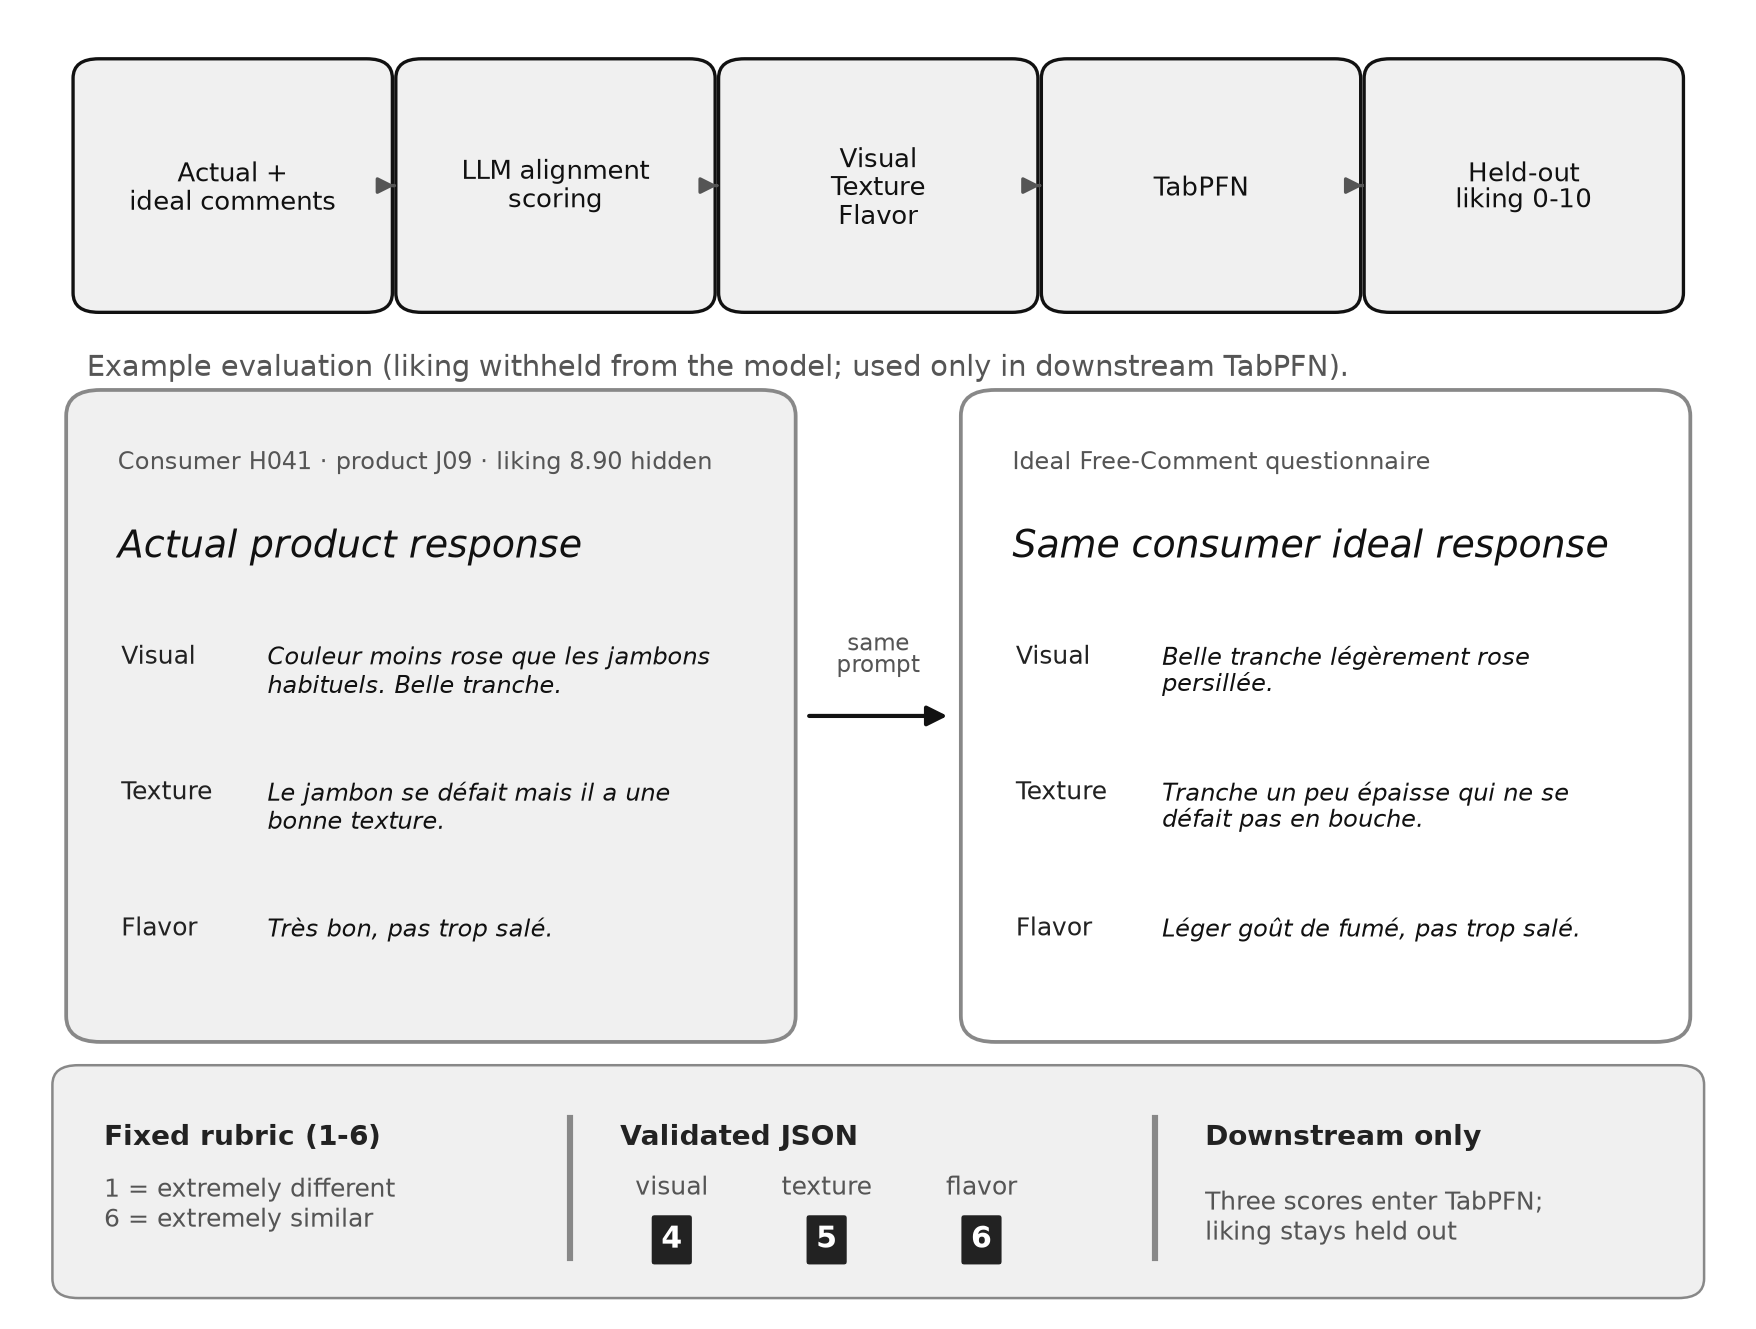
\includegraphics[width=\linewidth]{workflow_scoring.png}
\caption{Direct LLM alignment scoring. Top: pipeline from paired Free-Comment text to held-out liking. Bottom: example evaluation (liking withheld from the model) with fixed 1-6 rubric, validated JSON scores, and TabPFN inputs.}
\label{fig:workflow}
\end{figure}

\subsubsection{Response parsing and scoring reliability}
\label{sec:parsing}

Evaluations were scored and validated independently. The parser first
attempted direct JSON parsing, then used a regular-expression fallback for the
three expected fields. A response was accepted only if all three fields were
present and each score was an integer within the active scale range. For
thinking-enabled responses, any output parts flagged as model thought text were
skipped before parsing the answer. Each evaluation was attempted up to three
times at the API (Section~\ref{sec:models}), not as local re-parses of a single
response body.

No evaluation was dropped from modeling. If no valid response was obtained
within the retry budget, the three modality scores for that evaluation were
set to the scale midpoint, \texttt{(scale\_points + 1) // 2}, that is, the
lower of the two middle categories (2, 3, or 4 on the 4-, 6-, and 8-point
scales), so all 2,758 evaluations entered every downstream model. We report a scoring-error count
per configuration as a reliability indicator for the generation and parsing
loop: an evaluation was flagged if an API error, exception, or invalid
response occurred during its attempts, even when a later retry recovered a
valid score. In plain terms, the error count measures how often a
configuration failed to return a usable structured score on the first try. It
is a measure of operational reliability under a fixed schema, not a count of
excluded data and not a formal measure of task difficulty.

Configurations were also compared on operational criteria: wall-clock time for
a full scoring pass over all 2,758 evaluations, the scoring-error rate defined
above, and approximate API cost. We report cost qualitatively because provider
prices change; for scale, a full direct-response scoring pass completed in
about 100 seconds of wall-clock time at a cloud API cost that was small
relative to analyst time.

\subsection{Predicting liking from alignment scores}
\label{sec:prediction}

\subsubsection{Primary learner}
\label{sec:tabpfn}

For the primary predictive evaluation, only the three modality alignment
scores were used as predictors of 0--10 liking. The primary downstream learner
was TabPFN, a tabular foundation model trained on more than 100 million
synthetic tabular tasks generated from structural causal model priors
[Hollmann et al., 2025]. TabPFN predicts on a new tabular dataset through
in-context inference rather than ordinary hyperparameter search, which suits
this workflow: the LLM produces compact tabular features, and TabPFN predicts
liking without the tuning burden that would complicate a 27-configuration grid
search with bootstrap validation. Liking prediction used TabPFN v2 via
\texttt{TabPFNRegressor} [Hollmann et al., 2025], with the device set to CUDA
when available and CPU otherwise and all other inference settings left at
library defaults. No separate hyperparameter search was performed.

\subsubsection{Validation design and metrics}
\label{sec:validation}

The validation design used a single consumer-group holdout split with
\texttt{GroupShuffleSplit(test\_size = 0.20, n\_splits = 1, random\_state =
42)}, grouping by consumer. This prevented evaluations from the same consumer
from appearing in both training and holdout sets. A bootstrap sensitivity
analysis [Efron, 1979] was run on the two best single-split configurations
from each model family, six configurations in all. It held the LLM scores
fixed, rescaled each modality score to a common 0--10 range, and averaged the
three values into a single alignment predictor. For each of 200 replicates,
consumers were resampled with replacement, a fresh 20\% consumer-group holdout
was drawn within the resampled data, and TabPFN was refit. The bootstrap
therefore quantifies sensitivity to the consumer sample and split. It does not
repeat the LLM scoring, and because it uses the averaged single predictor it
is reported separately from the primary three-feature result. Family-level
win probabilities pooled the 200 $R^2$ draws from each family's two selected
configurations and compared aligned draws.

Predictive performance is reported with the coefficient of determination
($R^2$) and the mean absolute error (MAE), computed over held-out evaluations:
\[
R^2 = 1 - \frac{\sum_i (y_i - \hat{y}_i)^2}{\sum_i (y_i - \bar{y})^2},
\qquad
\mathrm{MAE} = \frac{1}{n}\sum_i |y_i - \hat{y}_i|,
\]
where $i$ indexes held-out consumer-product evaluations, $y_i$ is the observed
liking for evaluation $i$, $\hat{y}_i$ is the predicted liking, and $\bar{y}$
is the mean observed liking. $R^2$ measures the share of liking variance the
model explains (accuracy), and MAE measures the average prediction error in
points on the 0--10 liking scale. Both metrics pool the held-out evaluations;
they are not computed on product means.

To compare the contributions of the three modality scores, we computed
permutation importance on the held-out evaluations
(\texttt{n\_repeats = 10}, \texttt{random\_state = 42}), averaged the
importances across the 27 grid configurations, and normalized them within
method for comparison with the published modality signal.

\subsubsection{Downstream learner sensitivity analysis}
\label{sec:learners}

As a sensitivity analysis, the same direct LLM scores were also evaluated with
Ridge Regression [Hoerl and Kennard, 1970], Random Forest [Breiman, 2001],
Gradient Boosting [Friedman, 2001], and XGBoost [Chen and Guestrin, 2016]. For
that comparison, scores were rescaled to a common 0--10 range before fitting:
\[
\frac{\mathrm{score} - 1}{\mathrm{scale\_points} - 1} \times 10.
\]
The conventional learners used fixed, off-the-shelf settings rather than a
nested hyperparameter search: Ridge \texttt{alpha = 1.0}; Random Forest
\texttt{n\_estimators = 100}, \texttt{max\_depth = 10},
\texttt{random\_state = 42}; Gradient Boosting \texttt{n\_estimators = 100},
\texttt{max\_depth = 5}, \texttt{random\_state = 42}; and XGBoost
\texttt{n\_estimators = 100}, \texttt{max\_depth = 5},
\texttt{random\_state = 42}. This design keeps the comparison focused on the
LLM scoring configuration rather than on separately optimized learner
families. A fully tuned comparison would require nested tuning within the
training portion of each consumer-group split.

\subsection{Generic embedding-similarity baseline}
\label{sec:embedding}

As a reference floor, we also predicted liking from generic embedding
similarity. This baseline converted text into vectors and measured geometric
closeness without asking any model for a sensory judgment. In the primary
analysis it used the provider \texttt{models/text-embedding-004} embedding
model (768-dimensional vectors) through the REST
\texttt{batchEmbedContents} endpoint with
\texttt{taskType = "SEMANTIC\_SIMILARITY"}. Comments were first reduced to
modality-specific sensory descriptors by a separate LLM extraction step
(\texttt{gemini-2.0-flash}) that retained only sensory terms for the target
modality; actual and ideal descriptor texts were embedded separately for each
modality; and cosine similarity was computed between the actual vector $a$ and
ideal vector $i$ for each modality:
\[
\cos(a,i) = \frac{a \cdot i}{\lVert a \rVert \lVert i \rVert}.
\]
The three cosine similarities then entered the same downstream prediction as
the alignment scores. This baseline did not enforce the visual/texture/flavor
alignment judgment and did not receive liking. It is included as a simple
reference floor, not as a tuned competitor. The reported $R^2 = 0.200$ is from
that text-embedding-004 run (documented in the primary analysis notebook). The
public archive also includes a separate EmbeddingGemma sensitivity experiment
with different features and results; those files are not the source of the
$0.200$ reference figure.

\subsection{Topic-level validation}
\label{sec:topicmethods}

The primary pipeline uses three alignment scores. To compare more directly
with the Mahieu et al. [2022] descriptor analysis, we also ran a topic-level
version with 17 topic-alignment scores grounded in the descriptor families
from Mahieu et al. [2022]. Topics covered overall visual match, color and
pinkness, fat and lean appearance, surface moisture and shine, slice
structure, overall texture, tenderness, firmness and rubberiness, dryness and
juiciness, fibrous pieces, thickness and chew, overall flavor, saltiness, ham
taste, smoky or spiced notes, blandness or insipid intensity, and off-notes or
aftertaste.

The topic-level run used the direct-response configuration
(\texttt{gemini-flash-lite-latest}), temperature 0.7, and a six-point scale.
Each evaluation was scored once on the 17 topics; the prompt allowed
\texttt{null} when neither the actual nor the ideal text gave enough evidence
for a topic. Of 2,758 source evaluations, 2,757 produced valid topic-level
scores; the single evaluation that failed to parse was excluded from topic
summaries.

Each topic score measures actual-versus-ideal alignment for that topic; these
are not descriptor citation counts. Evaluation-level topic correlations used
the consumer-product evaluation as the statistical unit and computed Spearman
correlations between each topic score and that evaluation's liking.
Product-level summaries averaged each topic score by product across consumers
and correlated those 30 product means with product mean liking. We did not
attempt to rerun the original MR-CA: the open dataset provides the raw
comments and liking scores but not the curated descriptor citation matrix of
Mahieu et al. [2022], and reconstructing that matrix would reintroduce the
manual text-processing pipeline this approach is meant to avoid. Instead, we
compared structure: the modality order and the rank agreement of matched topic
families. Topic-rank agreement compared the strengths of the Mahieu et al.
[2022] drivers, taken as absolute values and normalized to sum to one across
matched families, with the LLM topic-liking correlations transformed the same
way. We compare strength rather than sign because the two quantities have
different meanings: a descriptor-presence effect can be negative when an
undesirable descriptor is cited, while an actual-to-ideal alignment score can
be positive when an undesirable attribute is absent. Rank agreement is
summarized with Spearman's $\rho$ and Kendall's $\tau_b$, a rank correlation
that handles ties [Kendall, 1938], with a two-sided permutation test for
$\tau_b$.

For a topic-level predictive check, the 17 topic scores were used to predict
liking under the same consumer-group holdout. The full topic-level TabPFN fit
exceeded the memory available in the compute environment used for that run, so
this check used a Gradient Boosting regressor [Friedman, 2001] with
scikit-learn default settings (100 trees, maximum depth 3) and
\texttt{random\_state = 42} as a diagnostic fallback. It is an extension of the structural validation, not a replacement
for the primary three-feature TabPFN result.

Observed liking is treated throughout as the criterion variable, not as a
perfect ground truth for consumer preference. The study asks whether
LLM-derived actual-to-ideal alignment scores predict stated liking and recover
the published sensory structure; it does not assume that every liking response
is noise-free.

\subsection{Validation against held-out Just-About-Right ratings}
\label{sec:jarmethods}

Recovering the published modality and topic structure is reassuring, but
liking is part of the same study the structure came from, so agreement could
partly reflect a shared hedonic signal. The dataset also contains a separate
structured signal: the JAR ratings for color, fat, salt, and tenderness
(Section~\ref{sec:dataset}). These were collected as distinct questions, were
never included in any scoring prompt, and map onto four of the topic-alignment
scores (color and pinkness, fat and lean appearance, saltiness, and
tenderness). They therefore allow a prompt-held-out construct check from the
same study sessions: if the model read the open comments correctly, its
alignment score for an attribute should be highest when the consumer rated that
attribute just about right and should fall as the rating moves toward either
extreme. This is internal validation against ratings not shown to the model,
not an external dataset replication.

For each of the four attributes we computed mean LLM alignment by JAR level,
the Spearman correlation between alignment and the absolute JAR deviation
$|\mathrm{JAR}|$, and the signed correlation with JAR. To test attribute
specificity rather than a general hedonic halo, we also correlated every LLM
attribute score with every JAR attribute, giving a four-by-four matrix in
which a diagonal pattern indicates attribute-specific recovery. The primary
validation used the same direct-response six-point topic-level scores as
Section~\ref{sec:topicmethods}, joined to the JAR ratings on consumer and
product.

To ask whether thinking improves this recovery, we repeated the topic-level
scoring with the two thinking configurations from the main
grid (minimal and low thinking) at the same six-point scale and temperature
0.7, and recomputed the same recovery and specificity metrics for each
configuration. We also ran a prompt-sensitivity check on a fixed 250-evaluation
sample, scoring all three configurations under the baseline prompt and under a
more explicit rubric prompt written to favor deliberative scoring, to test
whether the order of configurations on JAR recovery was stable across prompts.

\subsection{Software and implementation}
\label{sec:software}

Analyses were implemented in Python 3.9.6. The embedding-baseline and
TabPFN environment recorded pandas 2.3.3, scikit-learn 1.6.1, TabPFN
(tabpfn 7.1.1; ModelVersion.V2), and PyTorch 2.8.0. Downstream learner
comparisons also used XGBoost via \texttt{XGBRegressor} where available; the
historical XGBoost package version was not recorded in the archived environment
metadata, so that secondary comparison is not exactly environment-reproducible.
The primary grid liking models used TabPFN library defaults with device set to
CUDA or CPU. LLM scoring and text embedding used a commercial API from one provider (Google Gemini when we ran the work).
Scoring scripts, configuration-level grid summaries, bootstrap outputs,
topic-level per-evaluation alignment scores, and figure generators are
archived in the public repository described in the Data and code availability
statement.

\section{Results}
\label{sec:results}

\subsection{Predictive performance across the scoring grid}
\label{sec:gridresults}

The best of the 27 grid configurations used the direct-response setting, a
six-point scale, and temperature 0.7. It reached $R^2 = 0.573$ and MAE = 1.22
on the main consumer-group holdout split. The bootstrap sensitivity analysis
for this configuration produced mean $R^2 = 0.504$ with a 95\% interval of
[0.429, 0.582]; as described in Section~\ref{sec:validation}, that analysis
uses the mean of the three normalized alignment scores as a single predictor,
so it is reported separately from the primary three-feature estimate. To avoid
confounding thinking style with scale size or temperature,
Table~\ref{tab:controlled} compares the three configurations at the same
six-point scale and temperature 0.7.

\begin{table}[H]
\centering
\caption{Controlled predictive and operational comparison at six points and temperature 0.7. Time is wall-clock time for a full scoring pass over 2,758 evaluations; scoring errors are evaluations with at least one failed generation or parse attempt (Section~\ref{sec:parsing}).}
\label{tab:controlled}
\begin{tabular}{L{1.9in}lllll}
\toprule
Configuration & Scale, temp. & $R^2$ & MAE & Time (s) & Scoring errors \\
\midrule
Embedding baseline & -- & 0.200 & 1.83 & $<$5 & 0 (0.0\%) \\
Direct-response & 6 pt, 0.7 & 0.573 & 1.22 & 101 & 114 (4.1\%) \\
Low thinking & 6 pt, 0.7 & 0.479 & 1.33 & 619 & 137 (5.0\%) \\
Minimal thinking & 6 pt, 0.7 & 0.451 & 1.36 & 133 & 209 (7.6\%) \\
\bottomrule
\end{tabular}
\end{table}

The full grid supports the same conclusion without relying on one scale
setting (Figure~\ref{fig:grid}). Direct-response cells had the highest
mean $R^2$ for the direct-response group and the best overall cell, and all nine
direct-response cells occupied nine of the top ten positions by $R^2$. The
best low-thinking cell used an eight-point scale and temperature 0.7, with
$R^2 = 0.518$ and MAE = 1.26, still below the best direct-response result; the
best minimal-thinking cell reached $R^2 = 0.465$. Bootstrap comparisons among
selected top cells favored the direct-response class, with estimated winning
probabilities of 99.3\% versus minimal thinking and 91.2\% versus low thinking
(Figure~\ref{fig:grid}). These are descriptive bootstrap comparisons of the
selected configurations, not multiplicity-adjusted tests of all 27 cells, and
not a claim that every future model will order the same way. Full
per-configuration results for all 27 setups are given in \ref{app:fullgrid}
and in the project archive.

Within the thinking-capable generation, more thinking did not behave as a
simple improvement. Low thinking was not worse than minimal thinking on
prediction; at the controlled setting it was somewhat better
(Table~\ref{tab:controlled}). Neither thinking level closed the gap to the
direct-response configuration.

\begin{figure}[H]
\centering
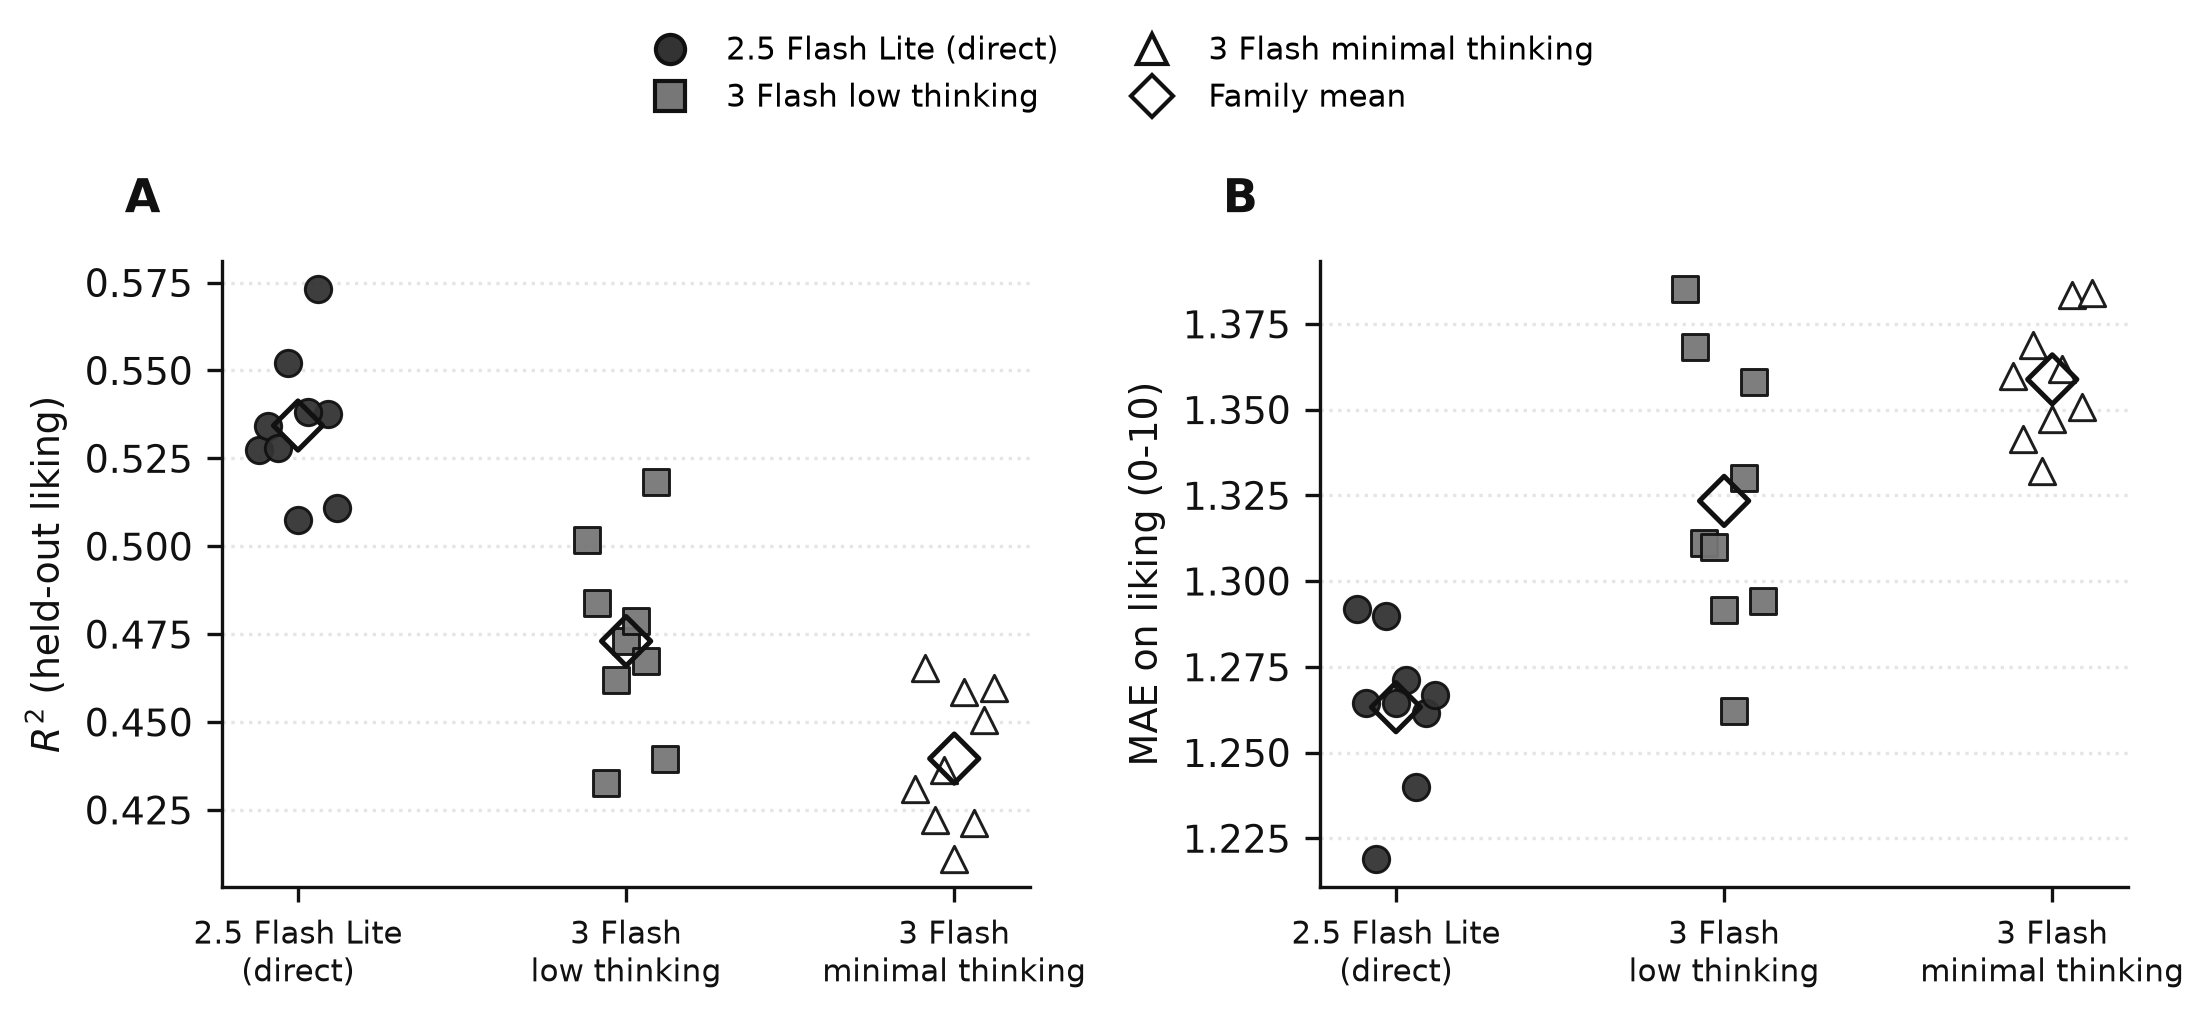
\includegraphics[width=\linewidth]{grid_performance.png}
\caption{Performance across the 27-configuration grid. Points are individual scale-by-temperature cells for each model configuration. (A) $R^2$ on held-out liking. (B) MAE on liking (0-10).}
\label{fig:grid}
\end{figure}

\subsection{Operational comparison}
\label{sec:opsresults}

The thinking configurations also carried operational costs
(Table~\ref{tab:controlled} and Figure~\ref{fig:ops}). Wall-clock time for a
full scoring pass rose from 101 seconds for the direct-response configuration
to 619 seconds at low thinking. At the same six-point scale and temperature
0.7, minimal thinking produced the most scoring errors (209 evaluations,
7.6\%, versus 114, 4.1\%, for direct-response). These failures matter because
the pipeline depends on thousands of parseable JSON responses; as noted in
Section~\ref{sec:parsing}, they measure operational reliability under a fixed
schema rather than task difficulty.

\begin{figure}[H]
\centering
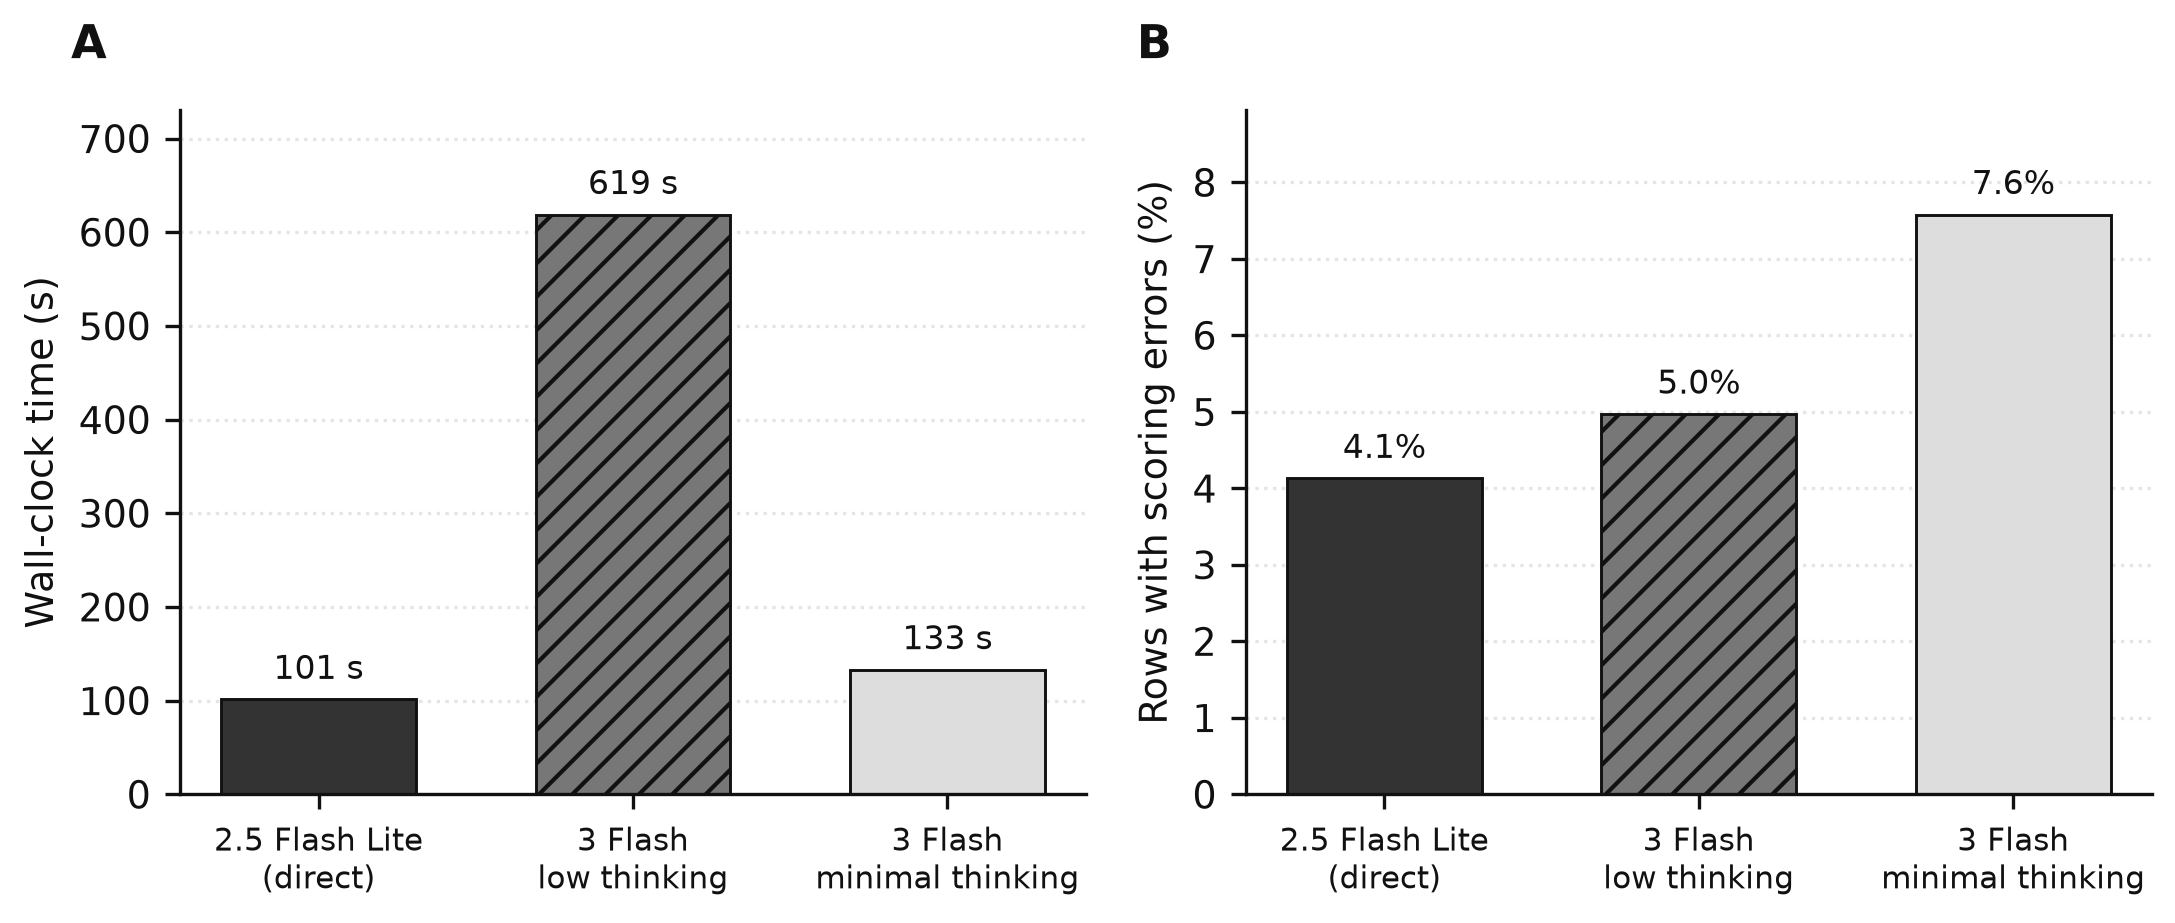
\includegraphics[width=\linewidth]{operational_comparison.png}
\caption{Operational comparison for the controlled six-point, temperature 0.7 configurations. A useful scorer must be accurate, fast enough to run across thousands of evaluations, and reliable enough to return parseable structured output.}
\label{fig:ops}
\end{figure}

\subsection{Comparison with the embedding baseline}
\label{sec:embeddingresults}

The generic embedding baseline reached $R^2 = 0.200$ and MAE = 1.83, well
below the $R^2 = 0.573$ of the best alignment-scoring configuration
(Table~\ref{tab:controlled}). This gap is informative because the task is more
than deciding whether two comments are semantically close. A consumer might
describe an actual ham and an ideal ham with overlapping words but different
sensory implications, and another consumer might use different words to
describe a close match. Raw cosine similarity does not force the comparison to
respect modality, hedonic direction, or consumer-specific ideals.

\subsection{Downstream learner comparison}
\label{sec:learnerresults}

The downstream learner comparison matters for the workflow rather than for the
headline result (Table~\ref{tab:learners}). Across the 27 LLM scoring
configurations, TabPFN had the best mean $R^2$ at 0.482 and won 20 of 27
configurations; Ridge Regression was the closest conventional baseline at
0.468. The conventional learners were untuned (Section~\ref{sec:learners}), so
this comparison shows that TabPFN is competitive and operationally convenient,
not that it is uniformly the best possible learner. The margin was modest, but
TabPFN required no separate hyperparameter search and runs as a single tabular
forward pass, which kept the 27-configuration grid and bootstrap loop
practical.

\begin{table}[H]
\centering
\caption{Downstream learner comparison across the 27 LLM scoring configurations. Conventional learners used fixed, untuned settings.}
\label{tab:learners}
\begin{tabular}{lll}
\toprule
Downstream learner & Mean $R^2$ & Configurations won \\
\midrule
TabPFN v2 & 0.482 & 20 (74.1\%) \\
Ridge Regression & 0.468 & 7 (25.9\%) \\
Gradient Boosting & 0.450 & 0 \\
Random Forest & 0.446 & 0 \\
XGBoost & 0.438 & 0 \\
\bottomrule
\end{tabular}
\end{table}

\subsection{Modality hierarchy and topic-level structure}
\label{sec:structureresults}

Permutation importance from the three-score model
(Section~\ref{sec:validation}) gave the largest
role to flavor, a smaller role to texture, and the weakest role to visual
appearance (Figure~\ref{fig:modality}). This matches the broad pattern in
Mahieu et al. [2022].

\begin{figure}[H]
\centering
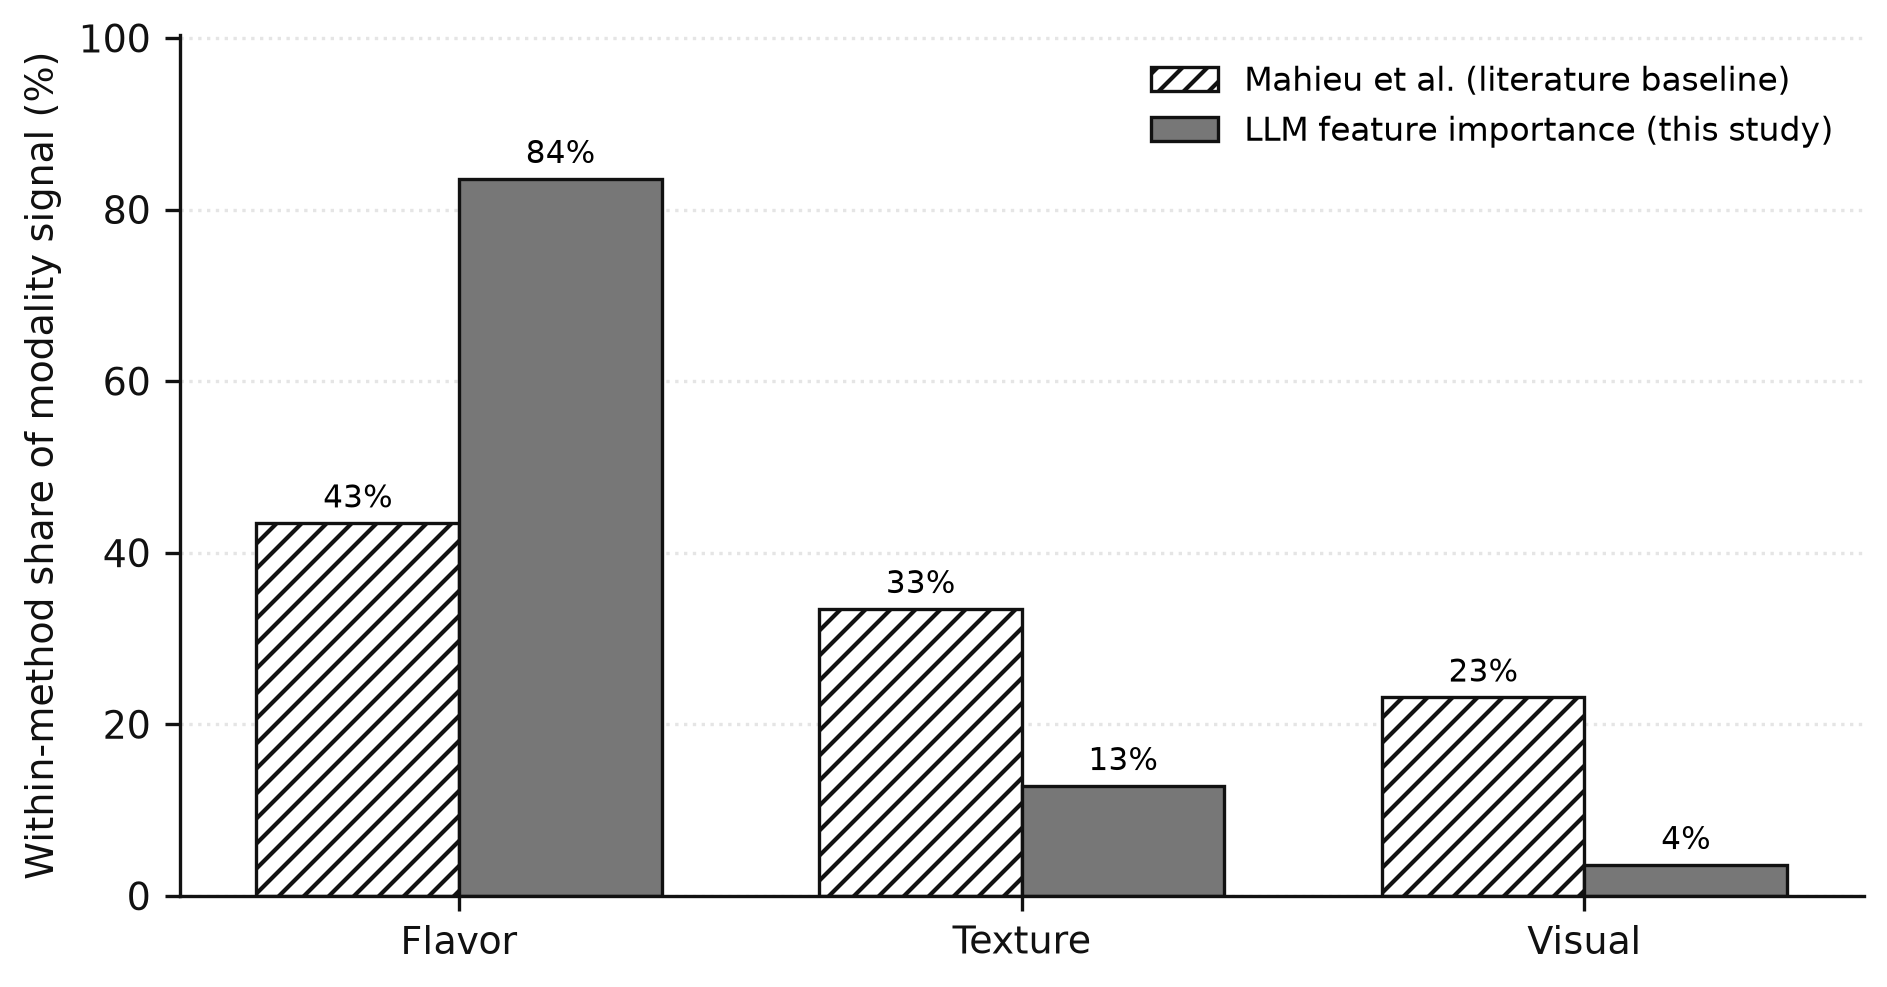
\includegraphics[width=0.93\linewidth]{modality_hierarchy.png}
\caption{Modality-level sanity check. Values are normalized within method so the comparison is about order and relative share, not raw units. Mahieu et al. [2022] values summarize modality signal from the original descriptor-based analysis, while our values are held-out permutation importances from the three LLM alignment scores, averaged across the 27 configurations.}
\label{fig:modality}
\end{figure}

The topic-level analysis strengthened that result (Table~\ref{tab:topic}). It
recovered the same modality order and showed substantial rank agreement across
matched topic families. Across 17 matched topic families, Kendall's $\tau_b$
was 0.519 with a two-sided permutation $p = 0.003$, Spearman's $\rho$ was
0.715, and nine of the ten strongest topic families in the original analysis
were also among the ten strongest LLM topic families
(Figure~\ref{fig:topicrank}). The topic-level predictive check with the
Gradient Boosting fallback reached $R^2 = 0.470$ and MAE = 1.37.

\begin{table}[H]
\centering
\caption{Topic-level validation results (direct-response configuration, six-point scale, temperature 0.7).}
\label{tab:topic}
\begin{tabular}{ll}
\toprule
Quantity & Result \\
\midrule
Valid topic-level evaluations & 2,757 \\
Unparsed evaluations & 1 \\
Topic families & 17 \\
Original modality order & Flavor $>$ Texture $>$ Visual \\
LLM modality order & Flavor $>$ Texture $>$ Visual \\
Modality Spearman $\rho$ & 1.000 \\
Topic rank Spearman $\rho$ & 0.715 \\
Topic rank Kendall $\tau_b$ & 0.519 \\
Topic-score liking prediction (GB fallback) & $R^2 = 0.470$; MAE = 1.37 \\
\bottomrule
\end{tabular}
\end{table}

\begin{figure}[H]
\centering
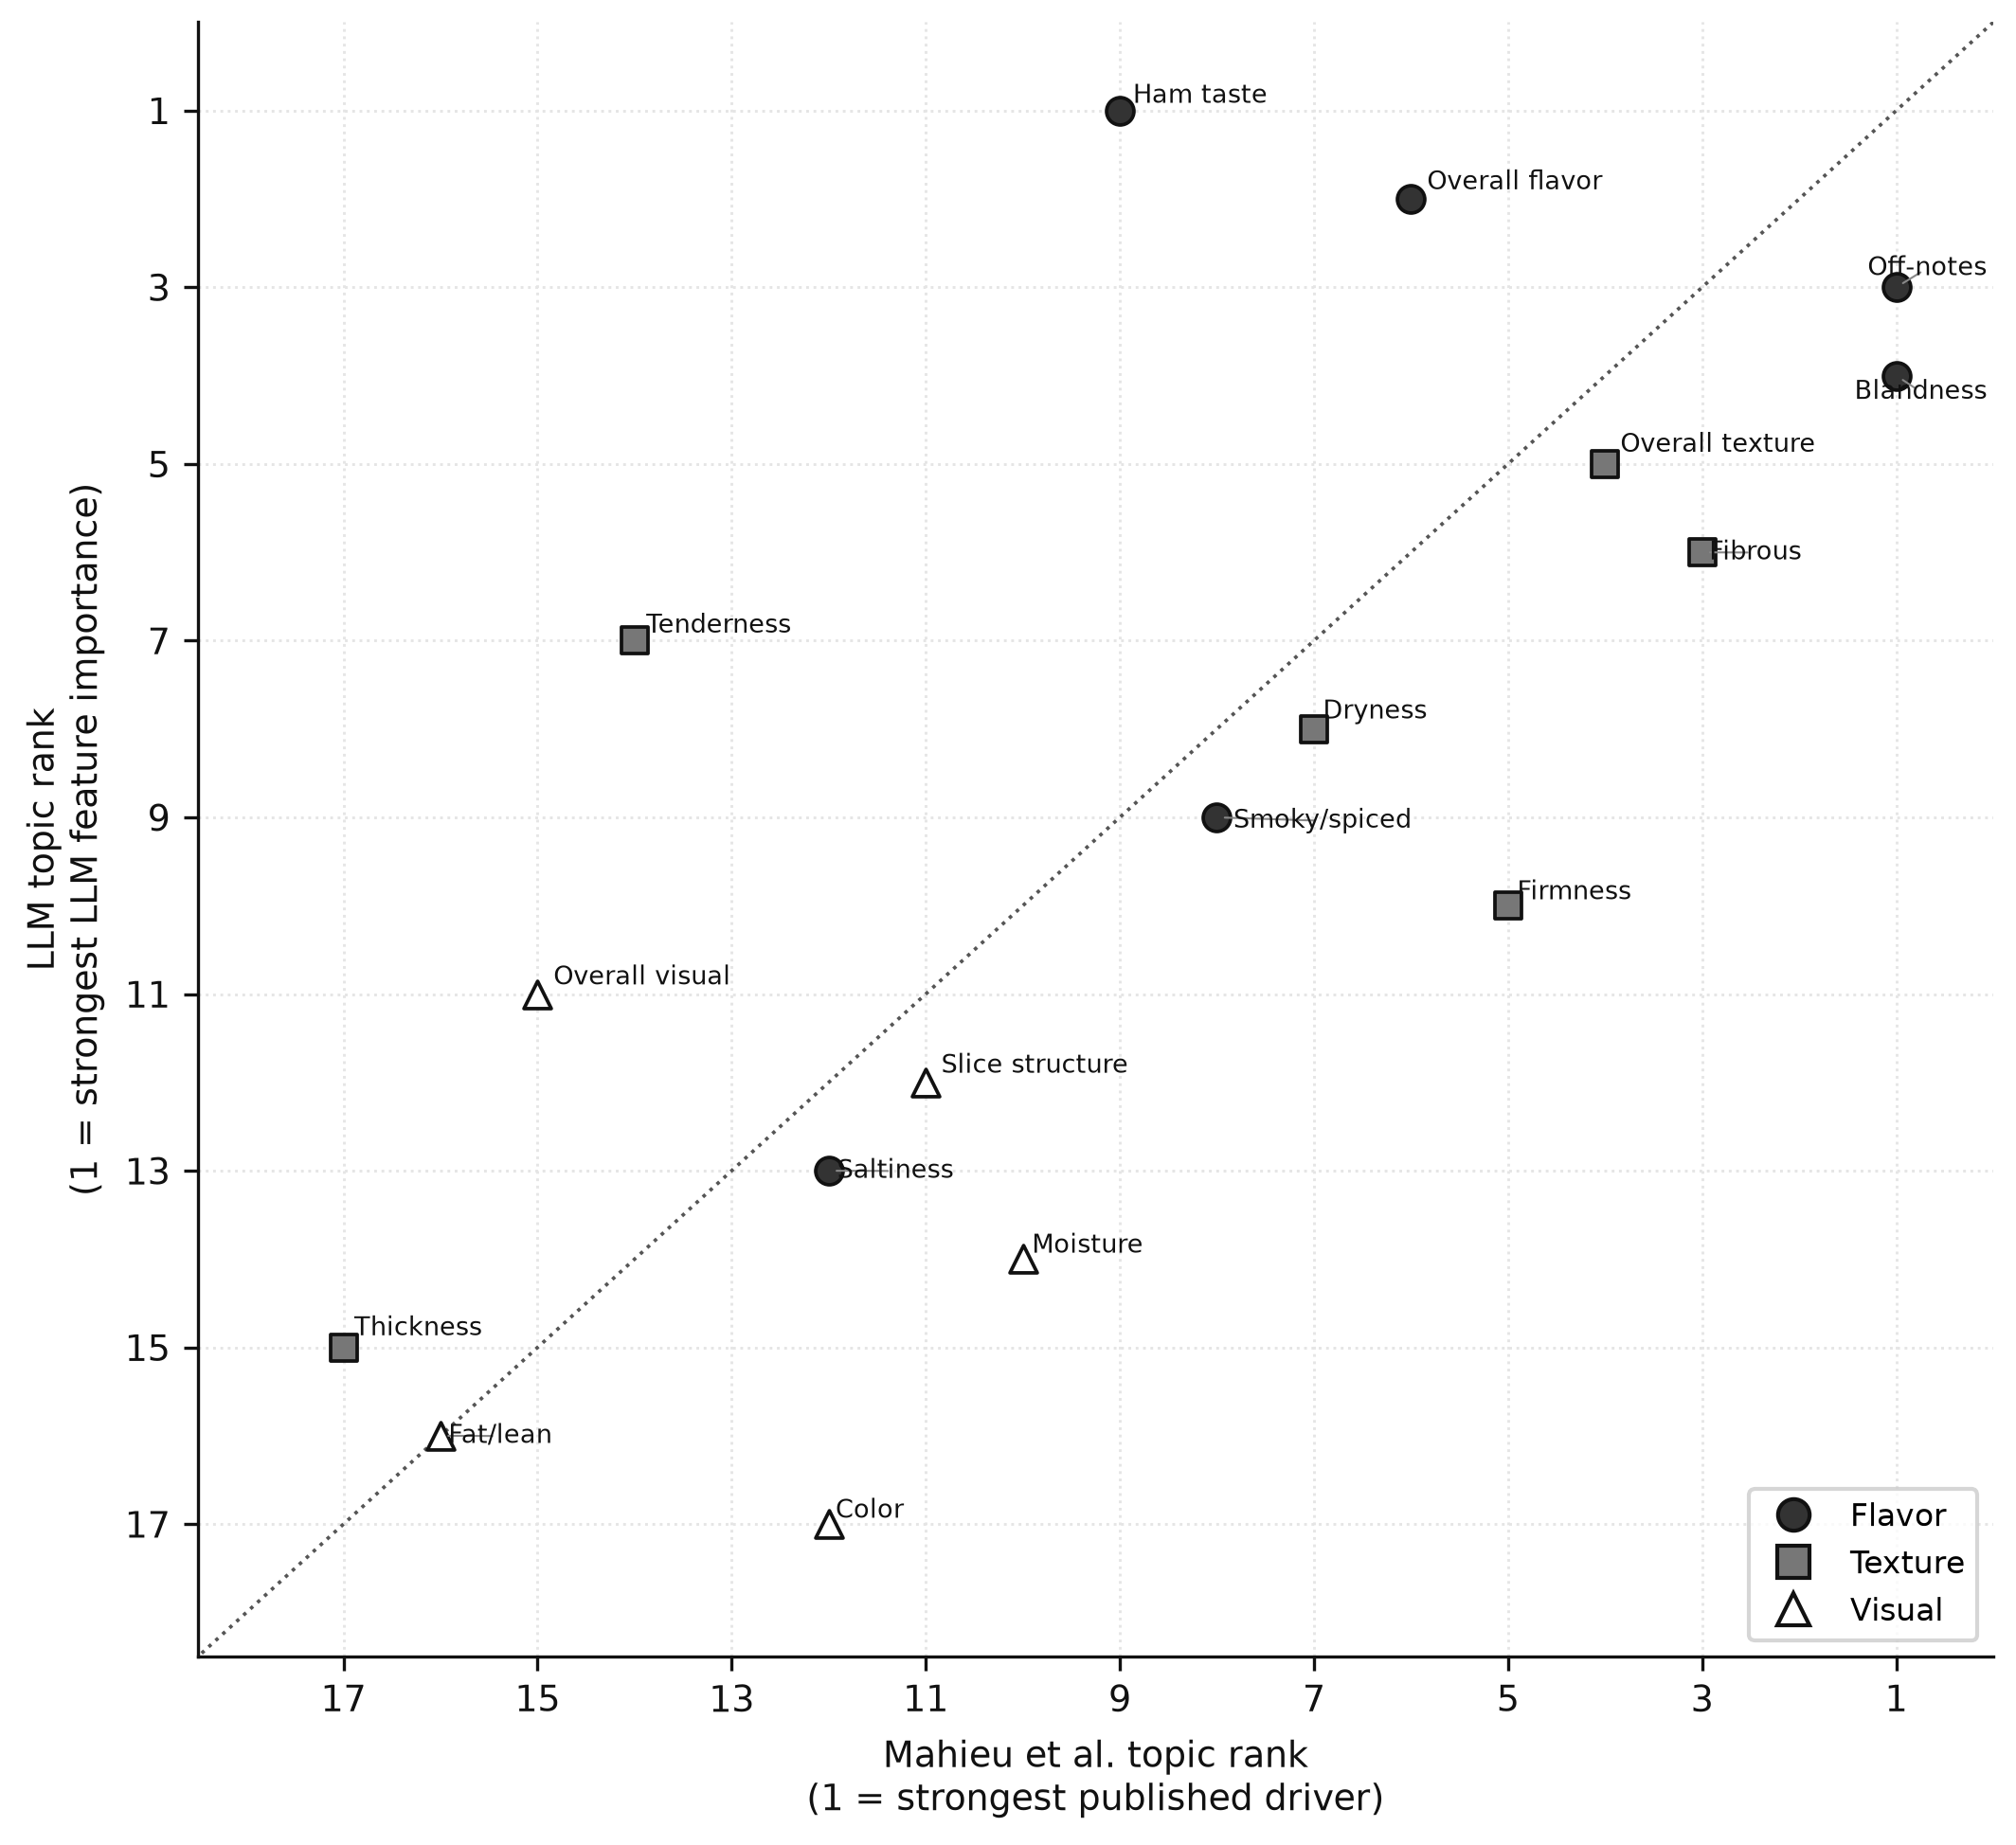
\includegraphics[width=0.86\linewidth]{topic_rank_comparison.png}
\caption{Rank-order comparison between mapped Mahieu et al. [2022] descriptor families and LLM topic-alignment families. Lower ranks are stronger. The comparison covers 17 matched topic families, with Kendall's $\tau_b = 0.519$ and Spearman's $\rho = 0.715$.}
\label{fig:topicrank}
\end{figure}

\subsection{Recovery of held-out Just-About-Right ratings}
\label{sec:jar}

The modality and topic-rank results above compare the LLM scores with
structure that was itself derived from liking. A stronger test uses the
held-out JAR ratings, which the model never saw. For all four attributes the
LLM alignment score peaked when the consumer rated the attribute just about
right and declined toward both the ``not enough'' and ``too much'' extremes,
the classic JAR tent shape (Figure~\ref{fig:jar}). The correlation between
alignment and absolute JAR deviation was negative for every attribute:
saltiness $\rho = -0.68$ ($n = 1{,}662$), tenderness $\rho = -0.59$
($n = 1{,}878$), fat and lean $\rho = -0.50$ ($n = 1{,}635$), and color
$\rho = -0.46$ ($n = 1{,}691$), all with nominal evaluation-level
$p < 10^{-10}$. The model recovered
these structured human judgments from free text it was only asked to compare
against each consumer's ideal.

\begin{figure}[H]
\centering
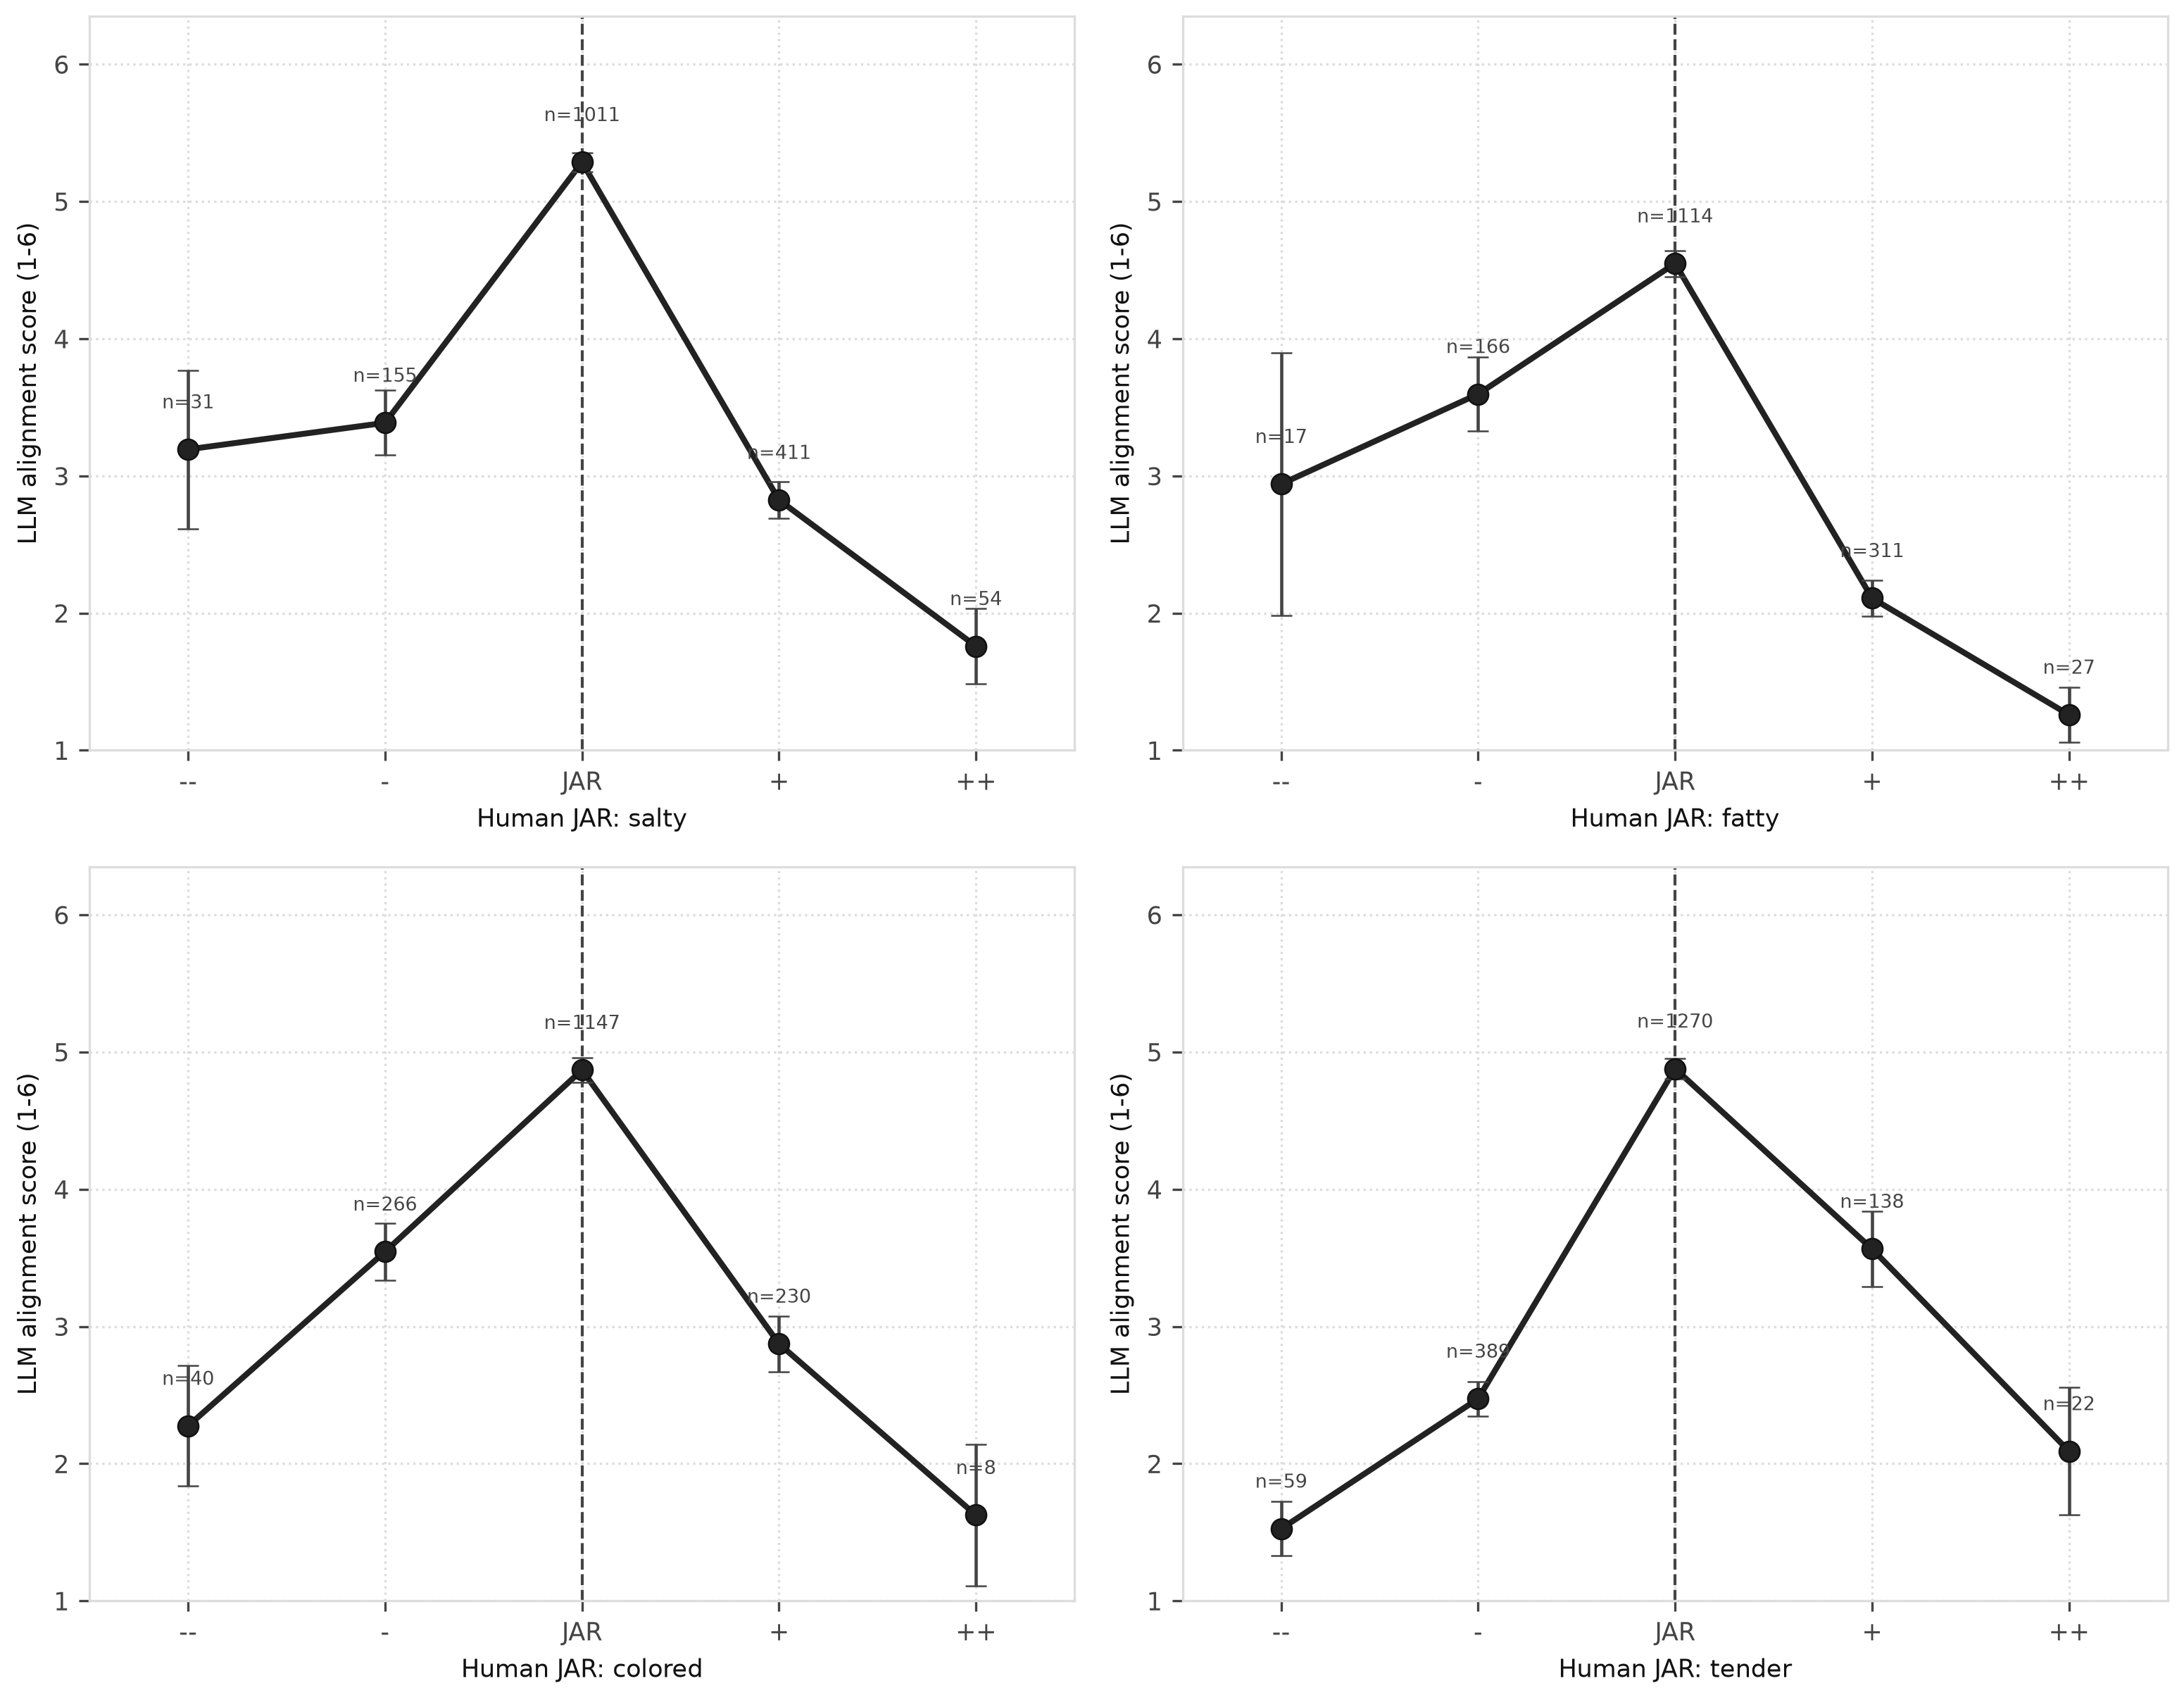
\includegraphics[width=\linewidth]{jar_validation.png}
\caption{LLM free-text alignment scores recover the human Just-About-Right structure. Each panel plots mean LLM alignment (1--6 similarity to the consumer's ideal) against the consumer's JAR rating for that attribute, from $-2$ (not enough) through 0 (just about right) to $+2$ (too much), with 95\% confidence intervals. The JAR ratings were never shown to the model.}
\label{fig:jar}
\end{figure}

The recovery was attribute-specific rather than a hedonic halo. Each LLM
attribute score tracked its own JAR rating more strongly than any other
(Table~\ref{tab:jarspec}): the mean matched (diagonal) correlation was
$-0.555$ against a mean mismatched correlation of $-0.251$, a specificity gap
of 0.30, and for every attribute the strongest recovery was its own JAR.

\begin{table}[H]
\centering
\caption{Attribute specificity. Spearman $\rho$ between each LLM attribute alignment score (rows) and each absolute JAR deviation (columns). More negative is stronger recovery; the diagonal is strongest in every row.}
\label{tab:jarspec}
\begin{tabular}{lcccc}
\toprule
LLM score & $|$JAR salt$|$ & $|$JAR fat$|$ & $|$JAR color$|$ & $|$JAR tender$|$ \\
\midrule
Saltiness   & \textbf{-0.68} & -0.23 & -0.25 & -0.24 \\
Fat / lean  & -0.24 & \textbf{-0.50} & -0.35 & -0.26 \\
Color       & -0.20 & -0.23 & \textbf{-0.45} & -0.20 \\
Tenderness  & -0.23 & -0.30 & -0.27 & \textbf{-0.59} \\
\bottomrule
\end{tabular}
\end{table}

The signed correlations recovered the deviation directions that matter for
cooked ham, in agreement with the drivers in Mahieu et al. [2022]. Alignment
fell faster on the ``too salty'' side than on the ``not salty enough'' side
(signed $\rho = -0.37$), and likewise for ``too fatty'' (signed
$\rho = -0.34$). For tenderness the penalized direction was ``not tender
enough'' (signed $\rho = +0.40$). Color was symmetric (signed
$\rho \approx 0$): both too pale and too dark reduced alignment. The model
therefore recovered which deviation direction lowers the match to the ideal
for each attribute, in addition to the overall tent shape.

Thinking did not improve this recovery. Scoring the same evaluations with the
two thinking configurations gave essentially the same result:
mean matched recovery was 0.555 for the direct-response configuration, 0.560
for minimal thinking, and 0.548 for low thinking, with comparable specificity
gaps (0.30 to 0.33) and comparable data completeness
(Figure~\ref{fig:jarcross}). The per-attribute correlations differed by at
most a few hundredths across configurations. The prompt-sensitivity check on a fixed 250-evaluation sample was consistent
with a near tie: minimal thinking ranked slightly first under both prompts,
while direct response and low thinking exchanged second and third place, and
each configuration's recovery moved by less than 0.02 between the baseline and
rubric prompts. This is descriptive agreement, not a formal equivalence test. The thinking
configurations were also far slower, with low thinking taking several times
the direct-response runtime. The direct-response configuration therefore
matched the thinking configurations at reading structured sensory judgments
out of free text; its advantage in the main analysis was specific to liking
prediction and to speed and reliability, not to attribute perception.

\begin{figure}[H]
\centering

\includegraphics[width=\linewidth]{cross_model_jar.png}
\caption{Cross-configuration JAR recovery. (A) Absolute Spearman correlation of alignment with $|\mathrm{JAR}|$ by attribute. (B) Mean matched recovery and specificity gap. Thinking configurations do not improve recovery relative to the direct-response configuration.}
\label{fig:jarcross}
\end{figure}

\subsection{Illustrative evaluation-level disagreements}
\label{sec:examples}

To make the aggregate contrast concrete, we inspected evaluations where the
configurations disagreed. In one high-liking case, consumer H041 gave the
product a liking score of 8.90. The actual comments included ``The ham breaks
apart, but it has a good texture'' and ``Very good, not too salty.'' The ideal
comments asked for a slightly thick slice that does not fall apart in the
mouth, is not too dry, and has a light smoky taste that is not too salty.

The two configurations received the same evaluation, prompt, and 1 to 6
similarity scale. The direct-response configuration scored the evaluation 4, 5, and 6 for visual,
texture, and flavor similarity to the ideal. The low-thinking configuration
scored it 4, 2, and 4. A plausible interpretation is that the thinking
configuration read the mention of the ham breaking apart as a severe literal
mismatch with the ideal slice description, while the direct-response
configuration weighted the consumer's overall positive sensory description.
Such examples do not replace the statistical results. They illustrate how a
more deliberative setup may over-read local mismatches in consumer language
(how the model scored the text, not the JSON parsing described in
Section~\ref{sec:parsing}) and convert them into severe similarity penalties
even when liking is high.

\section{Discussion}
\label{sec:discussion}

We began this work expecting the more deliberative configurations to be better
at this scoring job. The data pointed the other way. Among the setups we
tested, the best sensory scorer was the fast, direct-response configuration:
it predicted held-out liking better, ran roughly six times faster than the
low-thinking configuration, and returned parseable structured output more
reliably (Section~\ref{sec:gridresults} and Section~\ref{sec:opsresults}).
That reversal fits the nature of the target response. Liking a ham is a fast,
sensory, affective judgment. The scoring prompt asks the model to judge
whether the actual product matched the consumer's ideal experience, not to
solve a multi-step reasoning problem. In the dual-process analogy of
Section~\ref{sec:intro}, the task looks like a fast judgment, and the setup
matched to that regime measured it best. We treat this mapping as a hypothesis
for sensometrics, not as evidence about how models work inside. If sensory and
consumer tasks systematically favor different styles of inference,
model-cognition fit becomes a research program of its own for the field.

The comparison also gives a within-model reading. The two thinking
configurations differ only in thinking level, and moving from minimal to low
thinking did not behave as a simple improvement: low thinking was somewhat
better on prediction, the two were essentially tied on JAR recovery, and
neither closed the gap to the direct-response configuration
(Section~\ref{sec:gridresults} and Section~\ref{sec:jar}). The headline
direct-response versus thinking contrast confounds thinking with model
generation (Gemini 2.5 Flash Lite versus Gemini 3 Flash), as available at
scoring time (Section~\ref{sec:models}). That confound works against the
direct-response result rather than for it: the thinking cells used the newer
generation, and they still underperformed the older direct-response setup on
held-out liking, speed, and structured-output reliability. The clean
isolation of thinking level is the minimal-versus-low contrast within Gemini
3 Flash. We do not conclude that deeper thinking is generally better or
generally worse. We conclude that the thinking setting changed the
measurement, in cost and in quality, and that nothing about the more
deliberative options made them automatically superior. That is the finding a
researcher should carry into their own workflow: model settings matter, and
the direction of their effect on a given task is an empirical question.
Because LLM workflows are often judged as if capability were one-dimensional,
the natural default is to reach for the most advanced or most deliberative
option. On this task that default would have produced a slower, less accurate,
less reliable scorer.

Beyond the configuration contrast, direct LLM alignment scoring turned IFC
data into useful predictors of liking. The model received paired actual and
ideal consumer comments, scored sensory alignment, and produced tabular
features that predicted liking far better than generic embedding similarity
($R^2 = 0.573$ versus 0.200, Section~\ref{sec:embeddingresults}) and recovered
the same broad sensory hierarchy as the original descriptor-based analysis
(Section~\ref{sec:structureresults}). This complements the wider move toward
machine-learning prediction of liking from sensory data, such as the recent
prediction of coffee liking from sensory and JAR features [Gunning et al.,
2026]; the contribution here is that the predictors come directly from open
comments rather than from a pre-structured sensory table. The approach sits
between classical sensory statistics and newer LLM scoring methods. It keeps
the sensory structure of the problem, since the prompt asks for visual,
texture, and flavor comparisons and the topic-level extension uses families
grounded in the original descriptor analysis, while avoiding much of the
manual work of cleaning, lemmatizing, grouping, and filtering free comments
before modeling.

The method does change what is measured. Descriptor-presence analysis asks
what terms were cited and how their presence relates to liking. Alignment
scoring asks whether the actual product matched the consumer's ideal. These
are related but not identical targets, and signed descriptor coefficients
should not be compared one-to-one with our feature importances. The
appropriate comparison is broader structure: modality order and topic-rank
agreement, which is what Section~\ref{sec:structureresults} evaluates. For
liking prediction, the relational actual-versus-ideal score may be closer to
the consumer decision process than descriptor presence alone.

A natural concern is circularity: would a model that simply read the hedonic
tone of the actual comment track liking trivially? Three observations argue
against this. First, comparing each actual product against the consumer's own
ideal is the defining construct of IFC and of IPM [Mahieu et al., 2022, Worch
et al., 2013], not a quirk of the present workflow. Mahieu et al. [2022]
showed that ideals genuinely differ across consumers, separating the panel
into segments with opposite flavor ideals; a score that merely echoed the
actual comment could not exploit that consumer-specific reference. Second, the
recovery of the held-out JAR ratings was attribute-specific
(Section~\ref{sec:jar}): each alignment score tracked its own JAR attribute
far more strongly than the others, which a generic hedonic or sentiment
signal would not produce. Third, the generic embedding baseline operated on
the same actual and ideal text but reached only $R^2 = 0.200$, so the
predictive signal does not follow from the text alone but from the structured
actual-versus-ideal sensory judgment. Hedonic tone in the comments surely
contributes signal; the evidence indicates it is not the whole story.

These results also bear on the tradeoff between speed, cost, and evidence
quality that constrains consumer research. The original analysis required a
manual expert pipeline of cleaning, lemmatization, descriptor grouping,
frequency filtering, and cross-tabulation before any model could be fit, the
kind of preprocessing whose automation is itself under study [Visalli et al.,
2025a]. That pretreatment took an experienced analyst about half a day per
sensory modality, roughly two days in total including overhead, to turn the
raw comments into the descriptor table used for modeling. Direct alignment
scoring of all 2,758 evaluations took about 100 seconds of wall-clock time
with the direct-response configuration (Table~\ref{tab:controlled}), at a
cloud API cost that was small relative to that analyst time. The tradeoff does
not vanish; it moves. The recurring per-dataset cost of hand-coding
descriptors is replaced by a one-time engineering cost of prompt design,
calibration, and model versioning. The thinking-configuration results add a
caution to that engineering: spending more model compute per evaluation is not
where the measurement gains were found in this study.

The comparison should be treated as something that ages and needs rechecking.
Named API models move on quickly relative to peer review. That fact does not
weaken the result; it is why reported identifiers and scoring dates matter.
Model releases move the baseline, so a task-matched pilot
(Section~\ref{sec:recs}) should be rerun after major model changes, and
reported results should record the aliases, thinking settings, temperatures,
and scoring dates used. Judge-model and prompt choices are themselves sources
of measurement error in LLM workflows [Messing, 2026], which is a further
reason to keep the scoring loop auditable.

What should travel beyond this dataset is not a fixed ranking of Gemini
products. It is the demonstration that thinking level can matter, sometimes in
a surprising direction, on a sensory free-text task, together with a
model-cognition-fit account that invites further work. Other teams, using
other open or closed models and other product categories, should run their own
pilots rather than copy which setup ranked first for us. The analogy with
fast versus deliberate human judgment is offered as a prompt for further work,
not as a finished theory of how LLMs work.

\section{Recommendations for practice}
\label{sec:recs}

This paper does not recommend a specific commercial model. The commercial
models we used will be superseded, and a recommendation to adopt any named
system would be exactly the kind of blind default the results warn against.
What the results support is a discipline: before locking an LLM scoring
workflow for a full study, run a small task-matched pilot that varies thinking
level among other settings.

\begin{enumerate}
\item Define the judgment the model must make and the human signal that
validates it (here, actual-versus-ideal alignment validated against liking and
held-out JAR ratings).
\item Set aside a small sample of evaluations, including short, missing, and
contradictory comments, and hold everything constant except the model setup.
\item Compare setups, direct-response versus thinking levels, rather than
brand stories, and include at least one setup of each style.
\item Rank setups on task criteria: validity against the human signal,
structured-output reliability, runtime, and cost.
\item Prefer a prompt-held-out check the model never saw, as with the JAR
ratings here, over reusing the training signal.
\item Lock the winning setup with static model identifiers and a scoring date,
archive prompts and parsed scores, and re-check after major model releases.
\end{enumerate}

The pilot cost is small relative to a full study: in this work a full scoring
pass over 2,758 evaluations took about 100 seconds with the direct-response
configuration, and a pilot needs only a fraction of that. The same discipline
applies to open-weight and closed models alike. Choosing between them is a
research-management tradeoff involving access, cost, privacy, latency, and
reproducibility, and nothing in the fit idea is specific to closed systems.
Open-weight models offer stronger reproducibility guarantees because the
weights can be archived; the pilot loop above is how a team would establish
whether a given open or closed setup measures their task well.

\section{Limitations and future work}
\label{sec:limitations}

This is a single-product-category study. Cooked ham has a clear sensory
structure, and flavor dominates liking in the original analysis. Other
categories may have different modality balances and may not favor
direct-response configurations to the same extent.

A central limitation is scope of models. We stayed in one family of commercial
fast models (Gemini configurations when we ran the work) so that we could
explore thinking versus direct response without mixing provider stacks. That
design is useful for a controlled exploration; it is not a general survey of
LLMs. Open-weight models, other closed providers, and later generations may
order differently. Readers should treat our results as findings from this
exploration, not as universal. The scientific claim we stand behind is that
thinking level is worth testing on sensory text-scoring tasks, not that the
specific ranking of settings will hold for every laboratory.

Within that family the comparison spans a direct-response setup on Gemini 2.5
Flash Lite and two thinking levels on Gemini 3 Flash, the product slots
available for fast non-thinking versus thinking-capable scoring when we ran
the work. The headline contrast therefore confounds thinking setting with
generation and cannot attribute the gap to thinking alone; only the
minimal-versus-low contrast within Gemini 3 Flash isolates thinking level.
We chose those two thinking levels as the low end of the product dial for a
deployment-like cost and latency regime; higher thinking levels were not
tested. The confound does not rescue a weak direct-response model: if
anything, giving the thinking path the newer generation makes the failure of
extra thinking on this task more informative. Within the thinking-capable
generation at six points and temperature 0.7, low thinking improved
prediction and structured-output reliability relative to minimal thinking but
increased runtime, and neither closed the gap to the direct-response
configuration. Whether some task exists at which higher thinking levels would
dominate is an open question.

Because providers update aliases, what lasts is the pilot loop and the saved
scoring outputs. The public archive records the exact alias strings used, the
thinking configuration, the temperature, and the scoring date for each run,
together with configuration-level primary-grid summaries, topic-level
per-evaluation scores, and scripts that regenerate the reported downstream
tables from those fixed outputs. Rerunning live provider aliases is not
expected to reproduce the 15 January 2026 responses exactly. Other researchers
should run their own pilots on their own data rather than adopt our
configuration labels as a default.

Direct LLM alignment scoring is not SSR. SSR may provide better-calibrated
distributions and uncertainty information [Maier et al., 2025]. A fair
comparison should ask whether SSR's probability distributions improve
calibration or whether direct scoring wins because the prompt focuses the
model on the sensory comparison of interest.

The topic-level predictive check uses Gradient Boosting rather than TabPFN
because the full topic-level TabPFN fit exceeded available memory
(Section~\ref{sec:topicmethods}). It is a diagnostic extension of the
modality and topic-rank validation, not a replacement for the primary
three-feature TabPFN result. The topic-level comparison to Mahieu et al.
[2022] uses mapped descriptor families and driver strengths coded from the
published figure and processed notes, and should be read as a structural
validation of modality and topic order, not as a re-estimation of descriptor
coefficients.

The JAR validation is an internal construct check rather than a fully
external one. The JAR ratings were collected in the same study sessions as the
comments and liking ratings, so they share method variance, and topic scores were
null where the text gave no evidence for an attribute, leaving per-attribute
samples of roughly 1,600 to 1,900 evaluations. The evaluation-level
correlation tests also do not adjust for repeated consumers and products.
Replicating the JAR recovery
on an independent dataset is future work.

Headline prediction used a single consumer-group holdout after examining 27
configurations, and that search was not corrected for multiplicity. The
bootstrap resamples consumers and splits for six selected configurations,
holds the LLM scores fixed, and averages the three modality scores into one
predictor, so it does not repeat LLM generation, nest the configuration
selection, or provide an interval for the primary three-feature estimate.
Each configuration was scored once, including the temperature 0.7 runs, so
repeated-generation variability is not quantified, and the midpoint fallback
assigns the lower of the two middle categories, which could bias the few
affected evaluations slightly toward the different side. Repeated grouped
cross-validation and a pre-specified primary contrast would further harden
which setup ranks first, and a fully tuned comparison of downstream learners
would require nested tuning inside each training split; here TabPFN is
reported as competitive and convenient in practice rather than as the
uniformly best learner.

Finally, a model-person fit question is worth pursuing: whether some
consumers' comments are better scored by direct-response configurations and
others by more deliberative ones.

\section{Conclusion}
\label{sec:conclusion}

Direct LLM alignment scoring is a practical way to analyze Ideal-Free-Comment
data. In the cooked-ham case study it turned paired actual and ideal comments
into compact predictors of liking, outperformed generic embedding similarity,
recovered the main sensory hierarchy from the original Free-Comment analysis,
and recovered held-out Just-About-Right ratings attribute by attribute. Within
the Gemini family we used for this exploration, the best scorer among the
setups we tested was the direct-response setting. Setups with thinking turned
on were slower and did not close the predictive gap. That pattern held across
the configurations we ran, but it is a finding from this exploration, not a
general law. The point of the paper is that thinking level matters for sensory
free-text analysis, and that it can matter in a surprising way: more
deliberation was not automatically better. A simple comparison with how people
make fast sensory judgments versus more deliberate reasoning offers one
limited way to think about why that might be so; the human brain is far more
complex than any LLM, yet the parallel may open useful lines of research for
sensometricians. Other teams should try thinking settings on their own tasks
and tools, open or closed, rather than copy which setup ranked first for us.

\section*{Declaration of competing interest}

The authors declare no competing interests.

\section*{Declaration of generative AI and AI-assisted technologies in the manuscript preparation process}

During preparation of this manuscript, the authors used AI-assisted tools to
support literature synthesis, manuscript organization, drafting and review of
analysis code, and language editing. The human authors wrote, reviewed, and
edited the manuscript, take full responsibility for all scientific content,
analyses, and conclusions, and approved the final wording. All figures were
produced by the authors' own plotting code from the study's analysis outputs;
no figures or data were created or altered by generative image models.

\section*{Data and code availability}

Supporting materials for this paper (open consumer dataset used here,
configuration-level primary-grid summaries and bootstrap tables, topic-level
per-evaluation alignment scores, JAR validation outputs, analysis scripts,
figure generators, the primary scoring notebook, and manuscript sources) are
available at
\url{https://github.com/aigorahub/model-cognition-fit-supporting-materials}.
That repository exists only to support this manuscript. It is not a general
software product and does not include peer-review correspondence, credentials,
raw API response bodies, or private computing infrastructure.
Per-evaluation scores for the full 27-configuration primary grid are not
included, so that grid is auditable at the configuration-summary level;
topic-level analyses ship per-evaluation scores. A separate EmbeddingGemma
sensitivity folder is not the source of the manuscript's text-embedding-004
$R^2 = 0.200$ floor. Full re-scoring with a live model API is optional and
requires the reader's own credentials; the archived tables and scoring date
are the durable audit trail for the reported results.

\appendix

\section{Verbatim scoring prompt}
\label{app:prompt}

The exact prompt template used for all direct-scoring configurations was:

\begin{lstlisting}[language=Python]
def build_prompt(row, scale_points, scale_labels):
    """Build prompt with dynamic scale"""

    scale_text = "\n".join([f"  {i+1} = {label}" for i, label in enumerate(scale_labels)])

    prompt = f"""
You are a sensory and consumer scientist conducting consumer research on ham products.

TASK: Compare a consumer's ACTUAL ham experience to their IDEAL ham experience.
Score the alignment on each sensory dimension.

SCALE (1-{scale_points}):
{scale_text}

Focus only on sensory descriptions of the ham itself. Ignore any non-sensory comments.
Note: Responses are from French consumers and written in French.

IDEAL EXPERIENCE:
- Visual: {row.get('IdealVisual', '') or '(empty)'}
- Texture: {row.get('IdealTexture', '') or '(empty)'}
- Flavor: {row.get('IdealFlavor', '') or '(empty)'}

ACTUAL EXPERIENCE:
- Visual: {row.get('DescriptionVisual', '') or '(empty)'}
- Texture: {row.get('DescriptionTexture', '') or '(empty)'}
- Flavor: {row.get('DescriptionFlavor', '') or '(empty)'}

Return JSON only: {{"visual": X, "texture": X, "flavor": X}}
"""
    return prompt.strip()
\end{lstlisting}

The prompt inserted one of three ordered scales: a four-point scale (Very
Different; Somewhat Different; Somewhat Similar; Very Similar), a six-point
scale (Extremely Different; Very Different; Somewhat Different; Somewhat
Similar; Very Similar; Extremely Similar), or an eight-point scale (Extremely
Different; Very Different; Moderately Different; Slightly Different; Slightly
Similar; Moderately Similar; Very Similar; Extremely Similar).

\section{Full 27-configuration grid}
\label{app:fullgrid}

\small
\begin{longtable}{L{1.75in}rrrrrr}
\caption{Primary split results for all 27 direct alignment configurations. Configuration labels use the archive aliases for auditability; the scientific contrast is direct-response versus thinking level within one family of fast models at the time of scoring. Time is wall-clock seconds for a full scoring pass over 2,758 evaluations; errors are evaluations with at least one failed generation or parse attempt (Section~\ref{sec:parsing}).}\label{tab:fullgrid}\\
\toprule
Configuration & Scale & Temp. & $R^2$ & MAE & Time (s) & Errors \\
\midrule
\endfirsthead
\toprule
Configuration & Scale & Temp. & $R^2$ & MAE & Time (s) & Errors \\
\midrule
\endhead
Gemini 2.5 Flash Lite direct response & 4 & 0.0 & 0.5108 & 1.2919 & 102.3 & 118 \\
Gemini 2.5 Flash Lite direct response & 4 & 0.3 & 0.5274 & 1.2711 & 101.1 & 121 \\
Gemini 2.5 Flash Lite direct response & 4 & 0.7 & 0.5377 & 1.2644 & 101.2 & 126 \\
Gemini 2.5 Flash Lite direct response & 6 & 0.0 & 0.5342 & 1.2643 & 101.3 & 104 \\
Gemini 2.5 Flash Lite direct response & 6 & 0.3 & 0.5521 & 1.2399 & 101.3 & 112 \\
Gemini 2.5 Flash Lite direct response & 6 & 0.7 & 0.5731 & 1.2190 & 101.3 & 114 \\
Gemini 2.5 Flash Lite direct response & 8 & 0.0 & 0.5279 & 1.2616 & 103.9 & 109 \\
Gemini 2.5 Flash Lite direct response & 8 & 0.3 & 0.5075 & 1.2899 & 101.3 & 112 \\
Gemini 2.5 Flash Lite direct response & 8 & 0.7 & 0.5383 & 1.2669 & 100.6 & 114 \\
Gemini 3 Flash minimal thinking & 4 & 0.0 & 0.4214 & 1.3834 & 123.7 & 113 \\
Gemini 3 Flash minimal thinking & 4 & 0.3 & 0.4364 & 1.3689 & 124.9 & 125 \\
Gemini 3 Flash minimal thinking & 4 & 0.7 & 0.4111 & 1.3839 & 126.9 & 131 \\
Gemini 3 Flash minimal thinking & 6 & 0.0 & 0.4597 & 1.3507 & 137.3 & 196 \\
Gemini 3 Flash minimal thinking & 6 & 0.3 & 0.4654 & 1.3320 & 134.0 & 204 \\
Gemini 3 Flash minimal thinking & 6 & 0.7 & 0.4506 & 1.3618 & 133.0 & 209 \\
Gemini 3 Flash minimal thinking & 8 & 0.0 & 0.4311 & 1.3474 & 133.5 & 229 \\
Gemini 3 Flash minimal thinking & 8 & 0.3 & 0.4222 & 1.3599 & 134.1 & 232 \\
Gemini 3 Flash minimal thinking & 8 & 0.7 & 0.4586 & 1.3413 & 132.7 & 231 \\
Gemini 3 Flash low thinking & 4 & 0.0 & 0.4619 & 1.3580 & 547.8 & 85 \\
Gemini 3 Flash low thinking & 4 & 0.3 & 0.4327 & 1.3851 & 553.8 & 89 \\
Gemini 3 Flash low thinking & 4 & 0.7 & 0.4394 & 1.3683 & 582.6 & 87 \\
Gemini 3 Flash low thinking & 6 & 0.0 & 0.4730 & 1.3111 & 615.2 & 134 \\
Gemini 3 Flash low thinking & 6 & 0.3 & 0.4840 & 1.2917 & 614.6 & 128 \\
Gemini 3 Flash low thinking & 6 & 0.7 & 0.4787 & 1.3301 & 618.9 & 137 \\
Gemini 3 Flash low thinking & 8 & 0.0 & 0.4673 & 1.3098 & 669.5 & 154 \\
Gemini 3 Flash low thinking & 8 & 0.3 & 0.5019 & 1.2943 & 659.1 & 149 \\
Gemini 3 Flash low thinking & 8 & 0.7 & 0.5182 & 1.2620 & 666.4 & 155 \\
\bottomrule
\end{longtable}
\normalsize

\section*{References}

\noindent Argyle, L. P., Busby, E. C., Fulda, N., Gubler, J. R., Rytting, C.,
\& Wingate, D. (2023). Out of one, many: Using language models to simulate human
samples. \emph{Political Analysis}, 31(3), 337--351.
\url{https://doi.org/10.1017/pan.2023.2}.

\noindent Brand, J., Israeli, A., \& Ngwe, D. (2023). Using LLMs for market
research. Harvard Business School Working Paper 23-062.
\url{https://papers.ssrn.com/sol3/papers.cfm?abstract_id=4395751}.

\noindent Breiman, L. (2001). Random forests. \emph{Machine Learning}, 45(1),
5--32. \url{https://doi.org/10.1023/A:1010933404324}.

\noindent Califano, G., \& Caracciolo, F. (2026). Do large language models shop
like people? Comparing GPT and human food choices using discrete choice
experiments. \emph{Food Quality and Preference}, 142, 105930.
\url{https://doi.org/10.1016/j.foodqual.2026.105930}.

\noindent Chen, T., \& Guestrin, C. (2016). XGBoost: A scalable tree boosting
system. \emph{Proceedings of the 22nd ACM SIGKDD International Conference on
Knowledge Discovery and Data Mining}, 785--794.
\url{https://doi.org/10.1145/2939672.2939785}.

\noindent Efron, B. (1979). Bootstrap methods: Another look at the jackknife.
\emph{The Annals of Statistics}, 7(1), 1--26.
\url{https://doi.org/10.1214/aos/1176344552}.

\noindent Evans, J. St. B. T., \& Stanovich, K. E. (2013). Dual-process
theories of higher cognition: Advancing the debate. \emph{Perspectives on
Psychological Science}, 8(3), 223--241.
\url{https://doi.org/10.1177/1745691612460685}.

\noindent Friedman, J. H. (2001). Greedy function approximation: A gradient
boosting machine. \emph{The Annals of Statistics}, 29(5), 1189--1232.
\url{https://doi.org/10.1214/aos/1013203451}.

\noindent Garland, R. (1991). The mid-point on a rating scale: Is it
desirable? \emph{Marketing Bulletin}, 2, 66--70.

\noindent Gilardi, F., Alizadeh, M., \& Kubli, M. (2023). ChatGPT outperforms
crowd workers for text-annotation tasks. \emph{Proceedings of the National
Academy of Sciences}, 120(30), e2305016120.
\url{https://doi.org/10.1073/pnas.2305016120}.

\noindent Gema, A. P., H\"agele, A., Chen, R., et al. (2025). Inverse
Scaling in Test-Time Compute. \emph{Transactions on Machine Learning Research}.
\url{https://doi.org/10.48550/arXiv.2507.14417}.

\noindent Google. (2026). Gemini API documentation: Thinking.
\url{https://ai.google.dev/gemini-api/docs/thinking}. Accessed 2 August 2026.

\noindent Gunning, M., Serantes Laforgue, M. P., Guinard, J.-X., \& Tagkopoulos,
I. (2026). AI-driven prediction of consumer liking of coffee from sensory data.
\emph{npj Science of Food}, 10, 142.
\url{https://doi.org/10.1038/s41538-026-00779-7}.

\noindent Hamilton, L. M., \& Lahne, J. (2020). Fast and automated sensory
analysis: using natural language processing for descriptive lexicon development.
\emph{Food Quality and Preference}, 83, 103926.
\url{https://doi.org/10.1016/j.foodqual.2020.103926}.

\noindent Hamilton, K., Miller, R. J., \& Lahne, J. (2026). Sensory
applications of natural language processing and text analysis in practice: a
review of recent literature. \emph{Current Opinion in Food Science}, 67, 101370.
\url{https://doi.org/10.1016/j.cofs.2025.101370}.

\noindent Hoerl, A. E., \& Kennard, R. W. (1970). Ridge regression: Biased
estimation for nonorthogonal problems. \emph{Technometrics}, 12(1), 55--67.
\url{https://doi.org/10.1080/00401706.1970.10488634}.

\noindent Hollmann, N., M\"uller, S., Purucker, L., Krishnakumar, A., K\"orfer,
M., Hoo, S. B., Schirrmeister, R. T., \& Hutter, F. (2025). Accurate predictions
on small data with a tabular foundation model. \emph{Nature}, 637(8045),
319--326. \url{https://doi.org/10.1038/s41586-024-08328-6}.

\noindent Horton, J. J., Filippas, A., \& Manning, B. S. (2023). Large language
models as simulated economic agents: What can we learn from homo silicus? NBER
Working Paper 31122. \url{https://doi.org/10.3386/w31122}.

\noindent Jakkaew, P., Chondamrongkul, N., \& Suebsombut, P. (2026). LLM-Driven
Annotation: A scalable framework for automated multi-label coffee flavor
classification. \emph{ECTI Transactions on Computer and Information
Technology}, 20(2), 367--382.
\url{https://doi.org/10.37936/ecti-cit.2026202.264386}.

\noindent Kahneman, D. (2011). \emph{Thinking, Fast and Slow}. Farrar, Straus
and Giroux. ISBN: 9780374533557.

\noindent Kendall, M. G. (1938). A new measure of rank correlation.
\emph{Biometrika}, 30(1--2), 81--93.
\url{https://doi.org/10.1093/biomet/30.1-2.81}.

\noindent Liu, Y., Iter, D., Xu, Y., Wang, S., Xu, R., \& Zhu, C. (2023).
G-Eval: NLG evaluation using GPT-4 with better human alignment. \emph{Proceedings
of the 2023 Conference on Empirical Methods in Natural Language Processing},
2511--2522. \url{https://doi.org/10.18653/v1/2023.emnlp-main.153}.

\noindent Liu, R., Geng, J., Wu, A. J., Sucholutsky, I., Lombrozo, T., \&
Griffiths, T. L. (2024). Mind Your Step (by Step): Chain-of-Thought can Reduce
Performance on Tasks where Thinking Makes Humans Worse. Preprint,
arXiv:2410.21333. \url{https://arxiv.org/abs/2410.21333}.

\noindent Luc, A., L\^e, S., \& Philippe, M. (2020). Nudging consumers for
relevant data using Free JAR profiling: An application to product development.
\emph{Food Quality and Preference}, 79, 103751.
\url{https://doi.org/10.1016/j.foodqual.2019.103751}.

\noindent Mahieu, B., Visalli, M., Thomas, A., \& Schlich, P. (2020).
Free-comment outperformed check-all-that-apply in the sensory characterisation
of wines with consumers at home. \emph{Food Quality and Preference}, 84, 103937.
\url{https://doi.org/10.1016/j.foodqual.2020.103937}.

\noindent Mahieu, B., Schlich, P., Visalli, M., \& Cardot, H. (2021). A
multiple-response chi-square framework for the analysis of Free-Comment and
Check-All-That-Apply data. \emph{Food Quality and Preference}, 93, 104256.
\url{https://doi.org/10.1016/j.foodqual.2021.104256}.

\noindent Mahieu, B., Visalli, M., \& Schlich, P. (2022). Identifying drivers
of liking and characterizing the ideal product thanks to Free-Comment.
\emph{Food Quality and Preference}, 96, 104389.
\url{https://doi.org/10.1016/j.foodqual.2021.104389}.

\noindent Maier, B. F., Aslak, U., Fiaschi, L., Rismal, N., Fletcher, K.,
Luhmann, C. C., Dow, R., Pappas, K., \& Wiecki, T. V. (2025). LLMs reproduce
human purchase intent via semantic similarity elicitation of Likert ratings.
Preprint, arXiv:2510.08338.
\url{https://doi.org/10.48550/arXiv.2510.08338}.

\noindent Messing, S. (2026). Hidden measurement error in LLM pipelines
distorts annotation, evaluation, and benchmarking. Preprint, arXiv:2604.11581.
\url{https://arxiv.org/abs/2604.11581}.

\noindent Miller, C. A., Hamilton, L. M., \& Lahne, J. (2021). Sensory
descriptor analysis of whisky lexicons through the use of deep learning.
\emph{Foods}, 10(7), 1633. \url{https://doi.org/10.3390/foods10071633}.

\noindent Motoki, K., Low, J. Y. Q., \& Velasco, C. (2025). Generative AI
framework for sensory and consumer research. \emph{Food Quality and Preference},
133, 105600. \url{https://doi.org/10.1016/j.foodqual.2025.105600}.

\noindent OpenAI. (2024). Learning to reason with LLMs.
\url{https://openai.com/index/learning-to-reason-with-llms/}. Accessed
2 August 2026.

\noindent Rios de Souza, V., Popper, R., Plamenov, V., Wojnicz, P., \& Martinez,
J. (2024). Traditional preference mapping and computational machine learning
techniques: A comparative study of approaches to guide product development.
\emph{Food Quality and Preference}, 120, 105251.
\url{https://doi.org/10.1016/j.foodqual.2024.105251}.

\noindent Rupprecht, J., Ahnert, G., \& Strohmaier, M. (2025). Prompt
perturbations reveal human-like biases in large language model survey
responses. Preprint, arXiv:2507.07188.
\url{https://arxiv.org/abs/2507.07188}.

\noindent Sprague, Z., Yin, F., Rodriguez, J. D., Jiang, D., Wadhwa, M., Singhal,
P., et al. (2025). To CoT or not to CoT? Chain-of-thought helps mainly on
math and symbolic reasoning. \emph{International Conference on Learning
Representations (ICLR)}. \url{https://doi.org/10.48550/arXiv.2409.12183}.

\noindent Sui, Y., Chuang, Y.-N., Wang, G., Zhang, J., Zhang, T., Yuan, J.,
Liu, H., Wen, A., Zhong, S., Zou, N., Chen, H., \& Hu, X. (2025). Stop
Overthinking: A Survey on Efficient Reasoning for Large Language Models.
\emph{Transactions on Machine Learning Research}, accepted manuscript.
\url{https://doi.org/10.48550/arXiv.2503.16419}.

\noindent Symoneaux, R., Galmarini, M. V., \& Mehinagic, E. (2012). Comment
analysis of consumer's likes and dislikes as an alternative tool to preference
mapping. A case study on apples. \emph{Food Quality and Preference}, 24(1),
59--66. \url{https://doi.org/10.1016/j.foodqual.2011.08.013}.

\noindent ten Kleij, F., \& Musters, P. A. D. (2003). Text analysis of
open-ended survey responses: a complementary method to preference mapping.
\emph{Food Quality and Preference}, 14(1), 43--52.
\url{https://doi.org/10.1016/S0950-3293(02)00011-3}.

\noindent Torrico, D. D. (2025). The potential use of ChatGPT as a sensory
evaluator of chocolate brownies: a brief case study. \emph{Foods}, 14(3), 464.
\url{https://doi.org/10.3390/foods14030464}.

\noindent Turpin, M., Michael, J., Perez, E., \& Bowman, S. R. (2023). Language
models don't always say what they think: Unfaithful explanations in
chain-of-thought prompting. \emph{Advances in Neural Information Processing
Systems}, 36. \url{https://doi.org/10.48550/arXiv.2305.04388}.

\noindent Visalli, M., Mahieu, B., Thomas, A., \& Schlich, P. (2020). Automated
sentiment analysis of Free-Comment: An indirect liking measurement?
\emph{Food Quality and Preference}, 82, 103888.
\url{https://doi.org/10.1016/j.foodqual.2020.103888}.

\noindent Visalli, M., Loiseau, A.-L., Cordelle, S., Mahieu, B., \& Schlich, P.
(2024). A dataset of perception and preferences of French consumers for
commercial cooked hams sampled according to their nutritional values and claims.
\emph{Data in Brief}, 54, 110549. \url{https://doi.org/10.1016/j.dib.2024.110549}.

\noindent Visalli, M., Symoneaux, R., Mursic, C., Touret, M., Lourtioux, F.,
Coulibaly, K., \& Mahieu, B. (2025a). Can natural language processing or large
language models replace human operators for pre-processing word and
sentence-based free comments sensory evaluation data? \emph{Food Quality and
Preference}, 127, 105456. \url{https://doi.org/10.1016/j.foodqual.2025.105456}.

\noindent Visalli, M., Symoneaux, R., Mursic, C., Touret, M., Lourtioux, F.,
Coulibaly, K., \& Mahieu, B. (2025b). A dataset of annotated free comments on the
sensory perception of madeleines for benchmarking text mining techniques.
\emph{Data in Brief}, 58, 111250.
\url{https://doi.org/10.1016/j.dib.2024.111250}.

\noindent Visalli, M., \& Mahieu, B. (2023). Combining statistics and semantic
for an automated data analysis of Free-Comment sensory description of products.
15th Pangborn Sensory Science Symposium, Nantes, France. HAL: hal-04197590.
\url{https://hal.science/hal-04197590}.

\noindent Wang, Q. J., \& Pellegrino, R. (2025). Automating chemosensory
creativity assessment with large language models. \emph{Food Quality and
Preference}, 132, 105599.
\url{https://doi.org/10.1016/j.foodqual.2025.105599}.

\noindent Wei, J., Wang, X., Schuurmans, D., Bosma, M., Ichter, B., Xia, F.,
Chi, E., Le, Q., \& Zhou, D. (2022). Chain-of-thought prompting elicits
reasoning in large language models. \emph{Advances in Neural Information
Processing Systems}, 35. \url{https://doi.org/10.48550/arXiv.2201.11903}.

\noindent Worch, T., L\^e, S., Punter, P., \& Pag\`es, J. (2013). Ideal
Profile Method (IPM): the ins and outs. \emph{Food Quality and Preference},
28(1), 45--59. \url{https://doi.org/10.1016/j.foodqual.2012.08.001}.

\noindent Worch, T., \& Ennis, J. M. (2013). Investigating the single ideal
assumption using Ideal Profile Method. \emph{Food Quality and Preference},
29(1), 40--47. \url{https://doi.org/10.1016/j.foodqual.2013.01.005}.

\noindent Zheng, L., Chiang, W.-L., Sheng, Y., Zhuang, S., Wu, Z., Zhuang, Y.,
Lin, Z., Li, Z., Li, D., Xing, E. P., Zhang, H., Gonzalez, J. E., \& Stoica, I.
(2023). Judging LLM-as-a-judge with MT-Bench and Chatbot Arena. \emph{Advances
in Neural Information Processing Systems}. arXiv:2306.05685.
\url{https://arxiv.org/abs/2306.05685}.

\noindent Zhou, S., Ling, R., Chen, J., Wang, X., Fan, T., \& Wang, H. (2026).
When More Thinking Hurts: Overthinking in LLM Test-Time Compute Scaling.
Preprint, arXiv:2604.10739. \url{https://arxiv.org/abs/2604.10739}.

\end{document}
